% Options for packages loaded elsewhere
\PassOptionsToPackage{unicode}{hyperref}
\PassOptionsToPackage{hyphens}{url}
%
\documentclass[
]{book}
\usepackage{amsmath,amssymb}
\usepackage{lmodern}
\usepackage{iftex}
\ifPDFTeX
  \usepackage[T1]{fontenc}
  \usepackage[utf8]{inputenc}
  \usepackage{textcomp} % provide euro and other symbols
\else % if luatex or xetex
  \usepackage{unicode-math}
  \defaultfontfeatures{Scale=MatchLowercase}
  \defaultfontfeatures[\rmfamily]{Ligatures=TeX,Scale=1}
\fi
% Use upquote if available, for straight quotes in verbatim environments
\IfFileExists{upquote.sty}{\usepackage{upquote}}{}
\IfFileExists{microtype.sty}{% use microtype if available
  \usepackage[]{microtype}
  \UseMicrotypeSet[protrusion]{basicmath} % disable protrusion for tt fonts
}{}
\makeatletter
\@ifundefined{KOMAClassName}{% if non-KOMA class
  \IfFileExists{parskip.sty}{%
    \usepackage{parskip}
  }{% else
    \setlength{\parindent}{0pt}
    \setlength{\parskip}{6pt plus 2pt minus 1pt}}
}{% if KOMA class
  \KOMAoptions{parskip=half}}
\makeatother
\usepackage{xcolor}
\IfFileExists{xurl.sty}{\usepackage{xurl}}{} % add URL line breaks if available
\IfFileExists{bookmark.sty}{\usepackage{bookmark}}{\usepackage{hyperref}}
\hypersetup{
  pdftitle={Python para estadística},
  pdfauthor={Mario Alfonso Morales Rivera},
  hidelinks,
  pdfcreator={LaTeX via pandoc}}
\urlstyle{same} % disable monospaced font for URLs
\usepackage{color}
\usepackage{fancyvrb}
\newcommand{\VerbBar}{|}
\newcommand{\VERB}{\Verb[commandchars=\\\{\}]}
\DefineVerbatimEnvironment{Highlighting}{Verbatim}{commandchars=\\\{\}}
% Add ',fontsize=\small' for more characters per line
\usepackage{framed}
\definecolor{shadecolor}{RGB}{248,248,248}
\newenvironment{Shaded}{\begin{snugshade}}{\end{snugshade}}
\newcommand{\AlertTok}[1]{\textcolor[rgb]{0.94,0.16,0.16}{#1}}
\newcommand{\AnnotationTok}[1]{\textcolor[rgb]{0.56,0.35,0.01}{\textbf{\textit{#1}}}}
\newcommand{\AttributeTok}[1]{\textcolor[rgb]{0.77,0.63,0.00}{#1}}
\newcommand{\BaseNTok}[1]{\textcolor[rgb]{0.00,0.00,0.81}{#1}}
\newcommand{\BuiltInTok}[1]{#1}
\newcommand{\CharTok}[1]{\textcolor[rgb]{0.31,0.60,0.02}{#1}}
\newcommand{\CommentTok}[1]{\textcolor[rgb]{0.56,0.35,0.01}{\textit{#1}}}
\newcommand{\CommentVarTok}[1]{\textcolor[rgb]{0.56,0.35,0.01}{\textbf{\textit{#1}}}}
\newcommand{\ConstantTok}[1]{\textcolor[rgb]{0.00,0.00,0.00}{#1}}
\newcommand{\ControlFlowTok}[1]{\textcolor[rgb]{0.13,0.29,0.53}{\textbf{#1}}}
\newcommand{\DataTypeTok}[1]{\textcolor[rgb]{0.13,0.29,0.53}{#1}}
\newcommand{\DecValTok}[1]{\textcolor[rgb]{0.00,0.00,0.81}{#1}}
\newcommand{\DocumentationTok}[1]{\textcolor[rgb]{0.56,0.35,0.01}{\textbf{\textit{#1}}}}
\newcommand{\ErrorTok}[1]{\textcolor[rgb]{0.64,0.00,0.00}{\textbf{#1}}}
\newcommand{\ExtensionTok}[1]{#1}
\newcommand{\FloatTok}[1]{\textcolor[rgb]{0.00,0.00,0.81}{#1}}
\newcommand{\FunctionTok}[1]{\textcolor[rgb]{0.00,0.00,0.00}{#1}}
\newcommand{\ImportTok}[1]{#1}
\newcommand{\InformationTok}[1]{\textcolor[rgb]{0.56,0.35,0.01}{\textbf{\textit{#1}}}}
\newcommand{\KeywordTok}[1]{\textcolor[rgb]{0.13,0.29,0.53}{\textbf{#1}}}
\newcommand{\NormalTok}[1]{#1}
\newcommand{\OperatorTok}[1]{\textcolor[rgb]{0.81,0.36,0.00}{\textbf{#1}}}
\newcommand{\OtherTok}[1]{\textcolor[rgb]{0.56,0.35,0.01}{#1}}
\newcommand{\PreprocessorTok}[1]{\textcolor[rgb]{0.56,0.35,0.01}{\textit{#1}}}
\newcommand{\RegionMarkerTok}[1]{#1}
\newcommand{\SpecialCharTok}[1]{\textcolor[rgb]{0.00,0.00,0.00}{#1}}
\newcommand{\SpecialStringTok}[1]{\textcolor[rgb]{0.31,0.60,0.02}{#1}}
\newcommand{\StringTok}[1]{\textcolor[rgb]{0.31,0.60,0.02}{#1}}
\newcommand{\VariableTok}[1]{\textcolor[rgb]{0.00,0.00,0.00}{#1}}
\newcommand{\VerbatimStringTok}[1]{\textcolor[rgb]{0.31,0.60,0.02}{#1}}
\newcommand{\WarningTok}[1]{\textcolor[rgb]{0.56,0.35,0.01}{\textbf{\textit{#1}}}}
\usepackage{longtable,booktabs,array}
\usepackage{calc} % for calculating minipage widths
% Correct order of tables after \paragraph or \subparagraph
\usepackage{etoolbox}
\makeatletter
\patchcmd\longtable{\par}{\if@noskipsec\mbox{}\fi\par}{}{}
\makeatother
% Allow footnotes in longtable head/foot
\IfFileExists{footnotehyper.sty}{\usepackage{footnotehyper}}{\usepackage{footnote}}
\makesavenoteenv{longtable}
\usepackage{graphicx}
\makeatletter
\def\maxwidth{\ifdim\Gin@nat@width>\linewidth\linewidth\else\Gin@nat@width\fi}
\def\maxheight{\ifdim\Gin@nat@height>\textheight\textheight\else\Gin@nat@height\fi}
\makeatother
% Scale images if necessary, so that they will not overflow the page
% margins by default, and it is still possible to overwrite the defaults
% using explicit options in \includegraphics[width, height, ...]{}
\setkeys{Gin}{width=\maxwidth,height=\maxheight,keepaspectratio}
% Set default figure placement to htbp
\makeatletter
\def\fps@figure{htbp}
\makeatother
\setlength{\emergencystretch}{3em} % prevent overfull lines
\providecommand{\tightlist}{%
  \setlength{\itemsep}{0pt}\setlength{\parskip}{0pt}}
\setcounter{secnumdepth}{5}
\usepackage{booktabs}
\renewcommand{\chaptername}{Cap\'itulo} 
\renewcommand{\bibname}{Bibliograf\'ia}
\renewcommand{\figurename}{Figura}
\renewcommand{\tablename}{Tablas}
\renewcommand{\appendixname}{Ap\'endice}
\renewcommand{\contentsname}{Contenido}
\renewcommand{\indexname}{\'Indice tem\'atico}
\renewcommand{\listtablename}{\'Indice de tablas}
\renewcommand{\listfigurename}{\'Indice de figuras}
\ifLuaTeX
  \usepackage{selnolig}  % disable illegal ligatures
\fi
\usepackage[]{natbib}
\bibliographystyle{plainnat}

\title{Python para estadística}
\author{Mario Alfonso Morales Rivera}
\date{2022-05-28}

\usepackage{amsthm}
\newtheorem{theorem}{Theorem}[chapter]
\newtheorem{lemma}{Lemma}[chapter]
\newtheorem{corollary}{Corollary}[chapter]
\newtheorem{proposition}{Proposition}[chapter]
\newtheorem{conjecture}{Conjecture}[chapter]
\theoremstyle{definition}
\newtheorem{definition}{Definition}[chapter]
\theoremstyle{definition}
\newtheorem{example}{Example}[chapter]
\theoremstyle{definition}
\newtheorem{exercise}{Exercise}[chapter]
\theoremstyle{definition}
\newtheorem{hypothesis}{Hypothesis}[chapter]
\theoremstyle{remark}
\newtheorem*{remark}{Remark}
\newtheorem*{solution}{Solution}
\begin{document}
\maketitle

{
\setcounter{tocdepth}{1}
\tableofcontents
}
\hypertarget{introducciuxf3n}{%
\chapter{Introducción}\label{introducciuxf3n}}

Estimado lector, este documento corresponde a mis notas de clase del curso \textbf{Estadística Básica con Python}, que oriento como docente en el Programa de Estadística, facultad de ciencias Básicas, en la \href{https://www.unicordoba.edu.co}{Universidad de Córdoba}. Como toda creación humana es imperfecta, y este documento no es la excepción, le pido el favor que me ayude a mejorarlo. Puede hacerlo reportando palabras mal escritas, errores de ortografía (que de seguro abundan), párrafos que usted considere que son confusos o poco claros, bloques de código que no funcionen como se espera, entre otros. Estaré altamente agradecido con su ayuda y le recompensaré invitándole a un buen café que yo mismo prepararé para usted. Este documento se compiló usando Bookdown \citep{R-bookdown} y la versión 3.9.7 de Python \citep{van1995python}.

\hypertarget{por-quuxe9-python}{%
\section{¿Por qué Python?}\label{por-quuxe9-python}}

Python se ha convertido en uno de los lenguajes de programación más populares en los últimos años, especialmente para crear sitios web utilizando sus numerosos marcos web, como Django. Python es lo que se denomina un lenguaje de secuencias de comandos, ya que se pueden usar para escribir pequeños programas o secuencias de comandos rápidos. Python se distingue por su gran y activa comunidad de computación científica. La adopción de Python para la computación científica tanto en aplicaciones industriales como en investigación académica ha aumentado significativamente desde principios de la década de 2000 \citep{McKinney}.
Para el análisis de datos, la computación interactiva, exploratoria y la visualización de datos, Python inevitablemente será comparable con muchos otros lenguajes y herramientas de programación comerciales y de código abierto de uso específico en estadística, como R, MATLAB, SAS, Stata y otros. En los últimos años, el soporte de biblioteca mejorado de Python (principalmente pandas) lo ha convertido en una sólida alternativa para las tareas de manipulación de datos. Combinado con la fortaleza de Python en la programación de propósito general, es una excelente opción como lenguaje único para crear aplicaciones centradas en datos.

\hypertarget{instalaciuxf3n-de-python}{%
\section{Instalación de Python}\label{instalaciuxf3n-de-python}}

Hay muchas versiones de Python disponibles en Internet para descargar e instalar de forma gratuita. En este libro usamos \href{https://www.anaconda.com/products/individual}{Anaconda}, que agrupa un conjunto de herramientas para trabajar ciencia de datos y aprendizaje automático (Machine Learning) usando Python y R en un computador personal. Anaconda, en su versión individual, desarrollada para usuarios independientes, es la plataforma preferida para hacer ciencia de datos, con mas de 25 millones de usuarios en todo el mundo.

Anaconda proporciona un repositorio basado en la nube donde puede encontrar e instalar más de 7500 paquetes de ciencia de datos y aprendizaje automático. Con el comando \texttt{conda-install}, puede comenzar a usar miles de paquetes de código abierto de Python, R, Conda, y muchos otros lenguajes.

La edición individual de Anaconda es una solución flexible de código abierto que proporciona las utilidades para crear, distribuir, instalar, actualizar y administrar software de manera multiplataforma. Conda facilita la gestión de múltiples entornos de datos que se pueden mantener y ejecutar por separado sin interferencias entre sí.

\textbf{Anaconda Navigator} es una interfaz gráfica de usuario que viene con la edición individual de Anaconda. Desde \textbf{Anaconda Navigator} es fácil lanzar aplicaciones, manejar paquetes y entornos sin necesidad de usar comandos en la terminal del sistema. Algunas aplicaciones disponibles en esta interfaz gráfica son:

\begin{itemize}
\item
  \href{https://www.spyder-ide.org}{Spyder}: Un entorno científico gratuito y de código abierto escrito en Python, para Python, diseñado por y para científicos, ingenieros y analistas de datos.
\item
  \href{https://jupyter.org}{JupyterLab}: Es un entorno de desarrollo interactivo basado en la web para \textbf{NoteBooks}, código y datos. Permite a los usuarios configurar y organizar trabajos en ciencia de datos, computación científica, reportes estadísticos y aprendizaje automático.
\item
  \href{https://numpy.org}{NumPy}: \citep{harris2020array} Es el paquete fundamental y necesario para el análisis de datos y la computación científica de alto rendimiento en Python.
\item
  \href{https://pandas.pydata.org/docs/getting_started/index.html}{Pandas}: \citep{mckinney2010data} Contiene estructuras de datos de alto nivel y herramientas de manipulación diseñadas para hacer que el análisis de datos sea rápido y fácil en Python. Pandas se basa en NumPy y facilita su uso en aplicaciones centradas en este paquete.\\
\item
  \href{https://scipy.org}{SciPy}: Es una colección de algoritmos matemáticos y funciones construidas sobre NumPy. Agrega un poder significativo a Python al proporcionar al usuario comandos y clases de alto nivel para manipular y visualizar datos.
\item
  \href{https://matplotlib.org}{Matplotlib}: Matplotlib es una librería para crear visualizaciones estáticas, animadas e interactivas en Python.
\item
  \href{https://docs.conda.io/projects/conda/en/latest/\#}{Conda}: Es un sistema de código abierto para la administración de paquetes y entornos que se ejecuta en Windows, macOS y Linux. Con Conda se pueden instalar, ejecutar y actualizar rápidamente los paquetes y sus dependencias. Fue creado para programas de Python, pero puede empaquetar y distribuir software para cualquier otro lenguaje.
\end{itemize}

Para instalar anaconda vaya a la \href{https://www.anaconda.com/products/individual}{página oficial}, y siga las instrucciones para la descarga e instalación que allí se encuentran. En caso de necesitar asesoría adicional para la instalación le recomiendo entrar a \href{https://www.youtube.com/results?search_query=instalar+anaconda+python+2021}{Youtube} y seguir algunos de los tutoriales que enseñan cómo hacer la instalación dependiendo de su sistema operativo. También puede buscar en páginas y blogs que ofrecen tutoriales con las instrucciones de instalación y configuración paso a paso.

\hypertarget{ejecuciuxf3n-de-cuxf3digo-python}{%
\subsection{Ejecución de código Python}\label{ejecuciuxf3n-de-cuxf3digo-python}}

Una vez se ha hecho la instalación de Anaconda, los usuarios de Windows y Mac, en el menú de aplicaciones, deben tener el ícono de \emph{Anaconda}, en el cual se da clic para ejecutar \texttt{anaconda-navigator}


\includegraphics[width=4.83in]{anacondaNavIcon}

luego de cargar \texttt{anaconda-navigator} se despliega una ventana donde aparecen, entre otros, los íconos que se muestran en la figura \ref{fig:IconosAnaconda} desde donde se pueden lanzar las aplicaciones.

\begin{figure}

\includegraphics[width=0.5\linewidth]{SpyderIcon2} 
\includegraphics[width=0.5\linewidth]{JupyterLabIcon2} 
\includegraphics[width=0.5\linewidth]{JupyterNotebookIcon2} 
\includegraphics[width=0.5\linewidth]{QtConsoleIcon} \caption{Anaconda Navigator: Algunas aplicaciones}\label{fig:IconosAnaconda}
\end{figure}

Se recomienda usar \texttt{Notebooks}, cuando además de escribir y ejecutar código se requiere documentarlo, es decir acompañarlo de texto (en formato Markdown), fórmulas matemáticas y ecuaciones, tablas de datos, gráficos, imágenes y en general contenido multimedia. Los \texttt{Notebooks} se pueden crear usando las aplicaciones \texttt{JupyterLab} o \texttt{Jupyter\ Notebook}. Si lo que desea es escribir y ejecutar código para resolver una tarea específica, es decir escribir \texttt{Scripts}, los cuales se guardan con extensión \texttt{.py} se recomienda usar \texttt{Spyder} y por último si el interés ejecutar código de manera interactiva, linea por lineas en la consola de Python se recomienda usar \texttt{Qt\ Console}.

Por último para verificar que Python está funcionando bien en su computadora, lance \texttt{QtConsole} y escriba

\begin{Shaded}
\begin{Highlighting}[]
\BuiltInTok{print}\NormalTok{(}\StringTok{"Hola Mundo"}\NormalTok{) }
\end{Highlighting}
\end{Shaded}

\begin{verbatim}
## Hola Mundo
\end{verbatim}

deberá aparece como en la figura \ref{fig:holamundo}

\begin{figure}
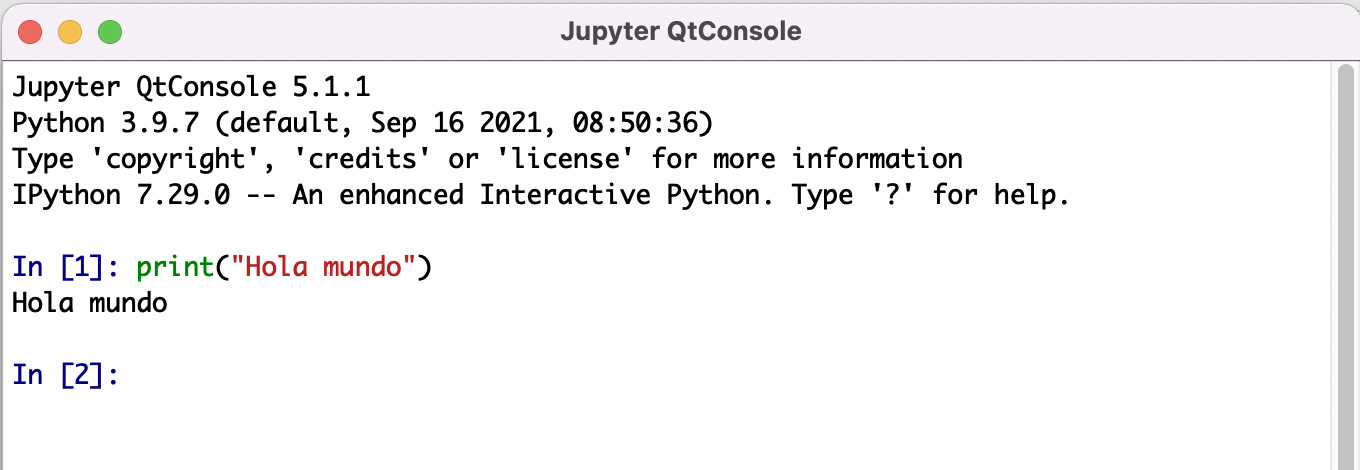
\includegraphics[width=0.95\linewidth]{HolaMundo} \caption{La primera línea de códido de todo programador}\label{fig:holamundo}
\end{figure}

\hypertarget{contenedores-de-datos-en-python}{%
\chapter{Contenedores de datos en Python}\label{contenedores-de-datos-en-python}}

Python ofrece varias estructuras para el almacenamiento de datos, entre ellas tenemos

\begin{itemize}
\tightlist
\item
  Tuplas \emph{(tuple)}
\item
  Listas \emph{(list)}
\item
  Arreglos \emph{(array)}
\item
  Diccionarios \emph{(dictionaries)}
\item
  Series \emph{(Series)}\\
\item
  Marcos de datos \emph{(DataFrames)}
\end{itemize}

Los arreglos que estudiaremos serán los definidos en el paquete \textbf{NumPy} \citep{harris2020array}, las \emph{Series} y \emph{data frames} no son del paquete estándar Python, en este curso usaremos las definidas en el paquete \emph{Pandas} \citep{mckinney2010data}.

\hypertarget{sec:tuplas}{%
\section{Tuplas}\label{sec:tuplas}}

Las tuplas se usan para agrupar objetos que pueden ser del mismo o de diferente tipo, son objetos indexados, iterables e \textbf{inmutables}, esta última propiedad implica que, una vez creadas, a las tuplas no se les puede modificar (agregar, quitar o cambiar entradas) .

\hypertarget{creaciuxf3n.}{%
\subsection{Creación.}\label{creaciuxf3n.}}

En esta sección estudiaremos como crear tuplas, acceder e iterar sobre sus elementos. En el siguiente bloque se crean e imprimen las tuplas \texttt{t1} y \texttt{t2}

\begin{Shaded}
\begin{Highlighting}[]
\NormalTok{t1}\OperatorTok{=}\NormalTok{(}\StringTok{\textquotesingle{}abc\textquotesingle{}}\NormalTok{,}\DecValTok{4}\NormalTok{,}\VariableTok{True}\NormalTok{,}\DecValTok{5}\NormalTok{,}\VariableTok{False}\NormalTok{,}\FloatTok{2.5}\NormalTok{,}\DecValTok{4}\NormalTok{,}\VariableTok{True}\NormalTok{,}\StringTok{"abc"}\NormalTok{,}\DecValTok{4}\NormalTok{,}\VariableTok{True}\NormalTok{,}\StringTok{"abc"}\NormalTok{)}\OperatorTok{;}\NormalTok{t1}
\end{Highlighting}
\end{Shaded}

\begin{verbatim}
## ('abc', 4, True, 5, False, 2.5, 4, True, 'abc', 4, True, 'abc')
\end{verbatim}

\begin{Shaded}
\begin{Highlighting}[]
\NormalTok{t2}\OperatorTok{=}\NormalTok{(}\DecValTok{1}\NormalTok{,}\FloatTok{0.7}\NormalTok{,t1,}\StringTok{"Hola"}\NormalTok{,}\DecValTok{4}\NormalTok{)}
\end{Highlighting}
\end{Shaded}

Observe que la tupla \texttt{t1} contiene elementos de tipo cadena de caracteres (str), números enteros (int), valores lógicos (bool) y valores reales o de punto flotante (floats). Incluso dentro de una tupla se pueden tener otras tuplas como ocurre con la tupla \texttt{t2} que tiene \emph{anidada} a la tupla \texttt{t1}.\\
Para acceder a los elementos de una tupla se usa \texttt{tupla{[}i{]}} donde \texttt{i} es un número entero entre cero (0) y la longitud de la tupla menos uno \((n-1)\). Por ejemplo, para recuperar elementos de la tupla \texttt{t1} usamos \texttt{t1{[}i{]}} con \texttt{i} entre cero y 11

\begin{Shaded}
\begin{Highlighting}[]
\NormalTok{t1[}\DecValTok{0}\NormalTok{] }\CommentTok{\# primer elemento de la tupla t1 }
\end{Highlighting}
\end{Shaded}

\begin{verbatim}
## 'abc'
\end{verbatim}

\begin{Shaded}
\begin{Highlighting}[]
\NormalTok{t1[}\DecValTok{2}\NormalTok{] }\CommentTok{\# tercer elemento de la tupla t1 }
\end{Highlighting}
\end{Shaded}

\begin{verbatim}
## True
\end{verbatim}

Esta característica común en todas las estructuras de datos indexadas con índice numérico en Python: el elemento \(k\) tiene índice \(k-1\), olvidar este hecho podria conducir a errores fatales.

Los usuarios de lenguajes como \texttt{R} o \texttt{MATLAB} podrían verse tentados a realizar la siguiente asignación

\begin{Shaded}
\begin{Highlighting}[]
\NormalTok{t1[}\DecValTok{2}\NormalTok{]}\OperatorTok{=}\DecValTok{0}
\end{Highlighting}
\end{Shaded}

buscando asignar el valor 0 al tercer elemento de la tupla, operacion que resultaría en el mensaje \texttt{TypeError:\ \ \textquotesingle{}tuple\textquotesingle{}\ object\ does\ not\ support\ item\ assignment}, a esta característica es que nos referimos con que las tuplas son \textbf{inmutables}, una vez creadas no es posible cambiar, eliminar, agregar elementos. Esta característica tiene por lo menos tres ventajas: proteje contra cambios accidentales en el contenido de la tupla, se gana eficiencia en cuanto al uso de memoria de la máquina y mayor rapidez de acceso a sus elementos.

Otra forma de crear tuplas es mediante la siguiente sintaxis, con la segunda linea se imprime el tipo de objeto que es \texttt{t3}, con el fin de verificar que efectivamente se ha creado una tupla.

\begin{Shaded}
\begin{Highlighting}[]
\NormalTok{t3}\OperatorTok{=}\DecValTok{10}\NormalTok{,}\DecValTok{20} 
\BuiltInTok{type}\NormalTok{(t3)  }
\end{Highlighting}
\end{Shaded}

\begin{verbatim}
## <class 'tuple'>
\end{verbatim}

Esta forma de crear tuplas se conoce como \emph{empaquetado}, también podemos recuperar los elementos de una tupla mediante el \emph{desempaquetado}, de la siguiente manera

\begin{Shaded}
\begin{Highlighting}[]
\NormalTok{x,y}\OperatorTok{=}\NormalTok{t3}
\BuiltInTok{print}\NormalTok{(}\StringTok{"x= "}\NormalTok{,x)}
\BuiltInTok{print}\NormalTok{(}\StringTok{"y= "}\NormalTok{,y)}
\end{Highlighting}
\end{Shaded}

el primer elemento de la tupla \texttt{t3} se asigna al objeto \texttt{x} y el segundo a \texttt{y} luego se imprimen sus valores. Se pueden crear tuplas vacías y tuplas que contiene un solo valor, llamadas tuplas unitarias como se muestra a continuación

\begin{Shaded}
\begin{Highlighting}[]
\NormalTok{tupvacia}\OperatorTok{=}\NormalTok{() }\CommentTok{\# crea una tupla vacía }
\NormalTok{tupunit}\OperatorTok{=}\NormalTok{(}\DecValTok{4}\NormalTok{,) }\CommentTok{\# crea una tupla con un único elemento }
\BuiltInTok{print}\NormalTok{(tupvacia,}\BuiltInTok{type}\NormalTok{(tupvacia),tupunit,}\BuiltInTok{type}\NormalTok{(tupunit))}
\end{Highlighting}
\end{Shaded}

\begin{verbatim}
## () <class 'tuple'> (4,) <class 'tuple'>
\end{verbatim}

note el uso de la coma después del elemento de la tupla unitaria, eso debe ser así porque de lo contrario no se estaría creando una tupla, sino un objeto de tipo entero (\texttt{int})

\begin{Shaded}
\begin{Highlighting}[]
\NormalTok{x}\OperatorTok{=}\NormalTok{(}\DecValTok{4}\NormalTok{) }\CommentTok{\# cuidado!!! x es un entero, no una tupla  }
\BuiltInTok{print}\NormalTok{(tupunit,}\BuiltInTok{type}\NormalTok{(tupunit))}
\end{Highlighting}
\end{Shaded}

\begin{verbatim}
## (4,) <class 'tuple'>
\end{verbatim}

\hypertarget{indexado-de-tuplas.}{%
\subsection{Indexado de tuplas.}\label{indexado-de-tuplas.}}

Se puede crear una tupla a partir de otra mediante órdenes de la forma \texttt{tupla{[}i:j{]}} esto se conoce como indexación, veamos algunos ejemplos:

\begin{Shaded}
\begin{Highlighting}[]
\NormalTok{a}\OperatorTok{=}\NormalTok{(}\DecValTok{3}\NormalTok{,}\DecValTok{2}\NormalTok{,}\DecValTok{4}\NormalTok{,}\DecValTok{1}\NormalTok{,}\DecValTok{6}\NormalTok{,}\DecValTok{4}\NormalTok{) }\CommentTok{\# se crea la tupla a }
\NormalTok{b}\OperatorTok{=}\NormalTok{a[}\DecValTok{1}\NormalTok{:}\DecValTok{4}\NormalTok{] }\CommentTok{\# tupla b, creada a partir de a }
\BuiltInTok{print}\NormalTok{(b,}\BuiltInTok{type}\NormalTok{(b))}
\end{Highlighting}
\end{Shaded}

\begin{verbatim}
## (2, 4, 1) <class 'tuple'>
\end{verbatim}

Note en la salida anterior que la tupla \texttt{b} inicia en \texttt{2}, y no en \texttt{3}, que es el primer elemento de la tupla \texttt{a} ¿por qué?

\begin{Shaded}
\begin{Highlighting}[]
\NormalTok{a[:}\DecValTok{4}\NormalTok{]    }\CommentTok{\# los cuatro primeros elementos de la tupla a}
\NormalTok{a[}\DecValTok{2}\NormalTok{:]    }\CommentTok{\# desde el tercer elemento hasta el final }
\NormalTok{a[::}\OperatorTok{{-}}\DecValTok{1}\NormalTok{]  }\CommentTok{\# la tupla en reversa  }
\end{Highlighting}
\end{Shaded}

\hypertarget{sec:funcionesAplicablesATuplas}{%
\subsection{Funciones y métodos aplicables a tuplas}\label{sec:funcionesAplicablesATuplas}}

La función \texttt{len()} regresa el número de elementos que contiene una tupla, el método \texttt{.index(x)} regresa el índice que le corresponde al elemento \texttt{x} en la tupla, si el elemento está más de una vez regresa el índice de la primera ocurrencia, en caso que \texttt{x} no esté ocurre un error. El método \texttt{.count()} regresa el número de veces que un elemento está en la tupla, en caso de no estar regresa creo, a continuación se muestra como usarlos sobre la tupla \texttt{t1} creada arriba

\begin{Shaded}
\begin{Highlighting}[]
\BuiltInTok{print}\NormalTok{(}\BuiltInTok{len}\NormalTok{(t1)) }\CommentTok{\# Imprime  la longitud  de la tupla}
\end{Highlighting}
\end{Shaded}

\begin{verbatim}
## 12
\end{verbatim}

\begin{Shaded}
\begin{Highlighting}[]
\NormalTok{t1[}\BuiltInTok{len}\NormalTok{(t1)}\OperatorTok{{-}}\DecValTok{1}\NormalTok{]  }\CommentTok{\# recupera el último elemento de la tupla t1}
\end{Highlighting}
\end{Shaded}

\begin{verbatim}
## 'abc'
\end{verbatim}

\begin{Shaded}
\begin{Highlighting}[]
\NormalTok{t1.index(}\DecValTok{4}\NormalTok{)    }\CommentTok{\# índice correspondiente al primer 4 en t1}
\end{Highlighting}
\end{Shaded}

\begin{verbatim}
## 1
\end{verbatim}

\begin{Shaded}
\begin{Highlighting}[]
\NormalTok{t1.count(}\DecValTok{4}\NormalTok{)    }\CommentTok{\# cuántas veces está 4 en t1 }
\end{Highlighting}
\end{Shaded}

\begin{verbatim}
## 3
\end{verbatim}

Habrá notado la diferencia en el llamado a \texttt{len()} frente a \texttt{.index()} y \texttt{.count()}: \texttt{len()} es una función genérica de Python , es independiente del objeto y puede aplicarse a diferentes tipos de objetos, mientras que los dos últimos son \emph{métodos}, definidos sobre la clase \emph{tuple}. Cuando se crea una tupla se le asocian los métodos propios de la clase, es decir, el método está asociado al objeto. Las funciones sólo se pueden llamar por su nombre, ya que se definen de forma independiente, pero los métodos no pueden ser llamados únicamente por su nombre, necesitamos invocar la clase por una referencia de esa clase en la que está definida. Esa es la razón por la que \textbf{no usamos} \texttt{index(t1,4)} o \texttt{count(t1,4)} sino \texttt{t1.index(4)} o \texttt{t1.count(4)} porque estos son métodos definidos sobre la clase \texttt{tuple}, mientras que \texttt{len()} es una función a la cual se le entrega una tupla y regresa su longitud, ella se puede usar con otros tipos de contenedores, incluso con cadenas de caracteres.

Para saber si un elemento hace parte de una tupla, usamos el operador \texttt{in} el cual regresa un valor lógico \texttt{True} o \texttt{False} dependiendo de si el elemento se encuentra o no en la tupla.

\begin{Shaded}
\begin{Highlighting}[]
\DecValTok{4} \KeywordTok{in}\NormalTok{ t1     }\CommentTok{\# True sí 4 está en t1, False si no  }
\end{Highlighting}
\end{Shaded}

\begin{verbatim}
## True
\end{verbatim}

\begin{Shaded}
\begin{Highlighting}[]
\CommentTok{"x"} \KeywordTok{in}\NormalTok{ t1   }\CommentTok{\# True sí  "x" está en t1,  False si no }
\end{Highlighting}
\end{Shaded}

\begin{verbatim}
## False
\end{verbatim}

\begin{Shaded}
\begin{Highlighting}[]
\CommentTok{"abc"} \KeywordTok{in}\NormalTok{ t1 }\CommentTok{\# True sí "abc" está en t1,  False si no }
\end{Highlighting}
\end{Shaded}

\begin{verbatim}
## True
\end{verbatim}

\hypertarget{operaciones-con-tuplas.}{%
\subsection{Operaciones con tuplas.}\label{operaciones-con-tuplas.}}

Se pueden concatenar y replicar tuplas usando los operadores \texttt{+} y \texttt{*} de la siguiente forma

\begin{Shaded}
\begin{Highlighting}[]
\NormalTok{Trats}\OperatorTok{=}\NormalTok{(}\StringTok{"T1"}\NormalTok{,}\StringTok{"T2"}\NormalTok{,}\StringTok{"T3"}\NormalTok{) }
\NormalTok{(}\DecValTok{2}\NormalTok{,}\DecValTok{3}\NormalTok{,}\DecValTok{4}\NormalTok{) }\OperatorTok{+}\NormalTok{ Trats }\CommentTok{\# Concatena la tupla (2,3,4) con Trats }
\end{Highlighting}
\end{Shaded}

\begin{verbatim}
## (2, 3, 4, 'T1', 'T2', 'T3')
\end{verbatim}

\begin{Shaded}
\begin{Highlighting}[]
\NormalTok{Trats}\OperatorTok{*}\DecValTok{3}         \CommentTok{\# replica la tupla Trats tres veces }
\end{Highlighting}
\end{Shaded}

\begin{verbatim}
## ('T1', 'T2', 'T3', 'T1', 'T2', 'T3', 'T1', 'T2', 'T3')
\end{verbatim}

\begin{Shaded}
\begin{Highlighting}[]
\NormalTok{(}\DecValTok{2}\NormalTok{,}\DecValTok{3}\NormalTok{,}\DecValTok{4}\NormalTok{)}\OperatorTok{*}\DecValTok{2}       \CommentTok{\# replica la tupla (2,3,4) tres veces }
\end{Highlighting}
\end{Shaded}

\begin{verbatim}
## (2, 3, 4, 2, 3, 4)
\end{verbatim}

\hypertarget{iterar-sobre-una-tupla.}{%
\subsection{Iterar sobre una tupla.}\label{iterar-sobre-una-tupla.}}

Una tupla es un objeto \emph{iterable}, es decir, se pueden recorrer uno tras otro sus elementos usando bucles, a continuación un ejemplo usando \texttt{for}

\begin{Shaded}
\begin{Highlighting}[]
\ControlFlowTok{for}\NormalTok{ i }\KeywordTok{in}\NormalTok{ Trats:}
    \BuiltInTok{print}\NormalTok{(i) }
\end{Highlighting}
\end{Shaded}

\begin{verbatim}
## T1
## T2
## T3
\end{verbatim}

\hypertarget{ejemplo-de-aplicaciuxf3n.}{%
\subsection{Ejemplo de aplicación.}\label{ejemplo-de-aplicaciuxf3n.}}

En el siguiente bloque de código se generan datos de una población normal con media cero y desviación estándar 10. Luego se usa la función \texttt{shapiro} para llevar a cabo la prueba de
\emph{Shapiro Wilks} sobre los datos. Lo que se quiere resaltar es que la función regresa una tupla que tiene como primer elemento el estadístico \(W\) y en la segunda posición el \(p-\)valor de la prueba, veamos

\begin{Shaded}
\begin{Highlighting}[]
\ImportTok{import}\NormalTok{ scipy.stats }\ImportTok{as}\NormalTok{ s  }
\ImportTok{import}\NormalTok{ numpy }\ImportTok{as}\NormalTok{ np}
\NormalTok{np.random.seed(seed}\OperatorTok{=}\DecValTok{123}\NormalTok{) }\CommentTok{\#\#\# para que el ejemplo sea reproducible }
\NormalTok{n }\OperatorTok{=}\NormalTok{ s.norm(}\DecValTok{0}\NormalTok{,}\DecValTok{10}\NormalTok{) }\CommentTok{\#se instancia una v.a normal de media 0 y sd 10}
\NormalTok{datos}\OperatorTok{=}\NormalTok{n.rvs(}\DecValTok{100}\NormalTok{) }\CommentTok{\# muestra de tamaño 100 de la normal }
\NormalTok{res}\OperatorTok{=}\NormalTok{s.shapiro(datos)  }
\CommentTok{\#print(res) \# se imprime la respuesta  }
\BuiltInTok{type}\NormalTok{(res) }\CommentTok{\# el tipo de objeto }
\end{Highlighting}
\end{Shaded}

\begin{verbatim}
## <class 'scipy.stats.morestats.ShapiroResult'>
\end{verbatim}

Note que \texttt{res}no es una tupla, pero se pueden recuperar los valores \(W\) y \(p\) mediante el desempaquetado o mediante el indexado como si lo fuera

\begin{Shaded}
\begin{Highlighting}[]
\NormalTok{W,p}\OperatorTok{=}\NormalTok{res  }\CommentTok{\# desempaquetado, equivalente a W=res[0] y p=res[1]}
\end{Highlighting}
\end{Shaded}

si estamos escribiendo un informe donde sea necesario reportar el resultado de la prueba podríamos usar

\begin{Shaded}
\begin{Highlighting}[]
\BuiltInTok{print}\NormalTok{(}\StringTok{"Estadístico de Shapiro {-} Wilks, }\SpecialCharTok{\%0.3f}\StringTok{, p\_valor = }\SpecialCharTok{\%0.4f}\StringTok{"} \OperatorTok{\%}\NormalTok{res)}
\end{Highlighting}
\end{Shaded}

\hypertarget{cuxf3mo-saber-si-un-objeto-de-python-es-una-tupla}{%
\subsection{¿Cómo saber si un objeto de Python es una tupla?}\label{cuxf3mo-saber-si-un-objeto-de-python-es-una-tupla}}

En algunas aplicaciones es necesario verificar si un objeto pertenece o no a una clase. Por ejemplo, para dirigir el flujo de ejecución del código de programación de una función: si el objeto entregado es una tupla, ejecute ciertas líneas de código, de lo contrario ejecute otras líneas. La función \texttt{isinstance(objeto,tipo)} regresa \texttt{True} si la clase del \texttt{objeto} entregado corresponde a \texttt{tipo}, en caso contrario regresa \texttt{False}.

\begin{Shaded}
\begin{Highlighting}[]
\BuiltInTok{isinstance}\NormalTok{(t1, }\BuiltInTok{tuple}\NormalTok{)}
\end{Highlighting}
\end{Shaded}

\begin{verbatim}
## True
\end{verbatim}

\begin{Shaded}
\begin{Highlighting}[]
\BuiltInTok{type}\NormalTok{(t1) }\KeywordTok{is} \BuiltInTok{tuple}
\end{Highlighting}
\end{Shaded}

\begin{verbatim}
## True
\end{verbatim}

Otra forma es usando la función \texttt{type()}, como se muestra a continuación

\begin{Shaded}
\begin{Highlighting}[]
\BuiltInTok{type}\NormalTok{(t1) }\KeywordTok{is} \BuiltInTok{tuple}
\end{Highlighting}
\end{Shaded}

\begin{verbatim}
## True
\end{verbatim}

\begin{Shaded}
\begin{Highlighting}[]
\BuiltInTok{type}\NormalTok{(}\DecValTok{4}\NormalTok{) }\KeywordTok{is} \BuiltInTok{tuple}
\end{Highlighting}
\end{Shaded}

\begin{verbatim}
## False
\end{verbatim}

esta última línea regresa \texttt{False} porque el número \texttt{4} no es una tupla. En las siguientes líneas se ilustra como indagar por los tipos de datos más usados en estadística

\begin{Shaded}
\begin{Highlighting}[]
\BuiltInTok{type}\NormalTok{(x) }\KeywordTok{is} \BuiltInTok{int}    \CommentTok{\# True si x es un entero False en caso que no}
\BuiltInTok{type}\NormalTok{(x) }\KeywordTok{is} \BuiltInTok{float}  \CommentTok{\# True si x es un real False en caso que no}
\BuiltInTok{type}\NormalTok{(x) }\KeywordTok{is} \BuiltInTok{str}    \CommentTok{\# True si x es un string  False en caso que no}
\BuiltInTok{type}\NormalTok{(x) }\KeywordTok{is} \BuiltInTok{bool}   \CommentTok{\# True si x es un lógico  False en caso que no}
\end{Highlighting}
\end{Shaded}

A manera de ejemplo, programar una función que reciba un objeto y en caso que este sea una tupla regrese el mensaje \texttt{\textquotesingle{}Es\ una\ tupla\textquotesingle{}} en caso contrario regrese \texttt{\textquotesingle{}No\ es\ una\ tupla\textquotesingle{}}

\begin{Shaded}
\begin{Highlighting}[]
\CommentTok{\# Se define la función }
\KeywordTok{def}\NormalTok{ verificartupla(x):}
  \ControlFlowTok{if}\NormalTok{(}\BuiltInTok{type}\NormalTok{(x) }\KeywordTok{is} \BuiltInTok{tuple}\NormalTok{):}
    \BuiltInTok{print}\NormalTok{(}\StringTok{"Es una tupla"}\NormalTok{)}
  \ControlFlowTok{else}\NormalTok{:}
    \BuiltInTok{print}\NormalTok{(}\StringTok{"No es una tupla"}\NormalTok{)}
\CommentTok{\# Fin de definición de función}
\end{Highlighting}
\end{Shaded}

\begin{Shaded}
\begin{Highlighting}[]
\CommentTok{\# Uso de  la función }
\NormalTok{verificartupla(t1) }\CommentTok{\# Retorna:  Es una tupla}
\NormalTok{verificartupla(}\StringTok{"hola"}\NormalTok{) }\CommentTok{\# Retorna:  No es una tupla}
\end{Highlighting}
\end{Shaded}

\hypertarget{ejercicios}{%
\subsection{Ejercicios}\label{ejercicios}}

\begin{enumerate}
\def\labelenumi{\arabic{enumi}.}
\tightlist
\item
  Escribir una función que reciba una tupla (se debe verificar que sea una tupla) y cuente cuántos elementos contiene de tipo \texttt{float} (reales), \texttt{int} (enteros), \texttt{str} (cadenas) y \texttt{bool} (lógicos). En caso de contener objetos de otro tipo los cuente como otros.
\item
  Escriba lineas de código Python que permita sumar los elementos numéricos de una tupla, por ejemplo para la tupla \texttt{(3,False,\textquotesingle{}x\textquotesingle{},2.5,1.5,\textquotesingle{}n\textquotesingle{})} se debe obtener \(3+2.5+1.5=7\).
\item
  Escriba lineas de código Python que permita promediar los elementos numéricos de una tupla.
\item
  Como se estudió en la sección \ref{sec:funcionesAplicablesATuplas}, el método \texttt{.index(val)} aplicado a una tupla regresa el índice donde por primera vez se encuentra \texttt{val}. Programe una función que tome una tupla y un valor, en caso que el valor esté en la tupla debe regresar una tupla que contenga los indices que le correspondan al valor entregado. Por ejemplo, si la tupla es \texttt{(9,5,2,6,5,3,8,5,3)} y el valor entregado es \texttt{5}, la función debe regresar \texttt{(1,4,7)}, la tupla con los índices que corresponden a \texttt{5}; si el valor entregado es 6, la función debe regresar la tupla unitaria \texttt{(3,)}; si el valor entregado es 4, la función debe imprimir el mensaje \texttt{4\ no\ está\ en\ la\ tupla}
\end{enumerate}

\hypertarget{sec:listas}{%
\section{Listas}\label{sec:listas}}

Las listas sirven para agrupar objetos de diferente tipo, aunque típicamente se usan para alojar datos de la misma naturaleza (números, caracteres, lógicos, \ldots), son indexadas y, a diferencia de las tuplas, son \textbf{mutables}, es decir, se les puede agregar, quitar y cambiar elementos después de creadas. Las listas soportan todas las características de las tuplas, pero es posible adicionar, remover y modificar sus elementos.

\hypertarget{creaciuxf3n}{%
\subsection{Creación}\label{creaciuxf3n}}

Para crear una lista colocamos los elementos dentro de corchetes de la siguente forma:

\begin{Shaded}
\begin{Highlighting}[]
\NormalTok{l1}\OperatorTok{=}\NormalTok{[}\OperatorTok{{-}}\DecValTok{5}\NormalTok{,}\OperatorTok{{-}}\DecValTok{4}\NormalTok{,}\OperatorTok{{-}}\DecValTok{3}\NormalTok{,}\OperatorTok{{-}}\DecValTok{2}\NormalTok{,}\OperatorTok{{-}}\DecValTok{1}\NormalTok{,}\DecValTok{1}\NormalTok{,}\DecValTok{2}\NormalTok{,}\DecValTok{3}\NormalTok{,}\DecValTok{4}\NormalTok{,}\DecValTok{5}\NormalTok{] }\CommentTok{\# lista de números enteros}
\NormalTok{l2}\OperatorTok{=}\NormalTok{[}\DecValTok{2}\NormalTok{,}\StringTok{"a"}\NormalTok{,}\VariableTok{True}\NormalTok{]    }\CommentTok{\#lista con elementos de distinto tipo}
\BuiltInTok{print}\NormalTok{(l2,}\BuiltInTok{type}\NormalTok{(l2))}
\end{Highlighting}
\end{Shaded}

\begin{verbatim}
## [2, 'a', True] <class 'list'>
\end{verbatim}

\hypertarget{IndexadoDeListas}{%
\subsection{Indexado de listas}\label{IndexadoDeListas}}

Cada elemento de una lista está asociado con un \emph{índice} que refleja su posición en el arreglo. Como en las tuplas, el primer elemento tiene índice 0, el segundo índice 1 y así sucesivamente. Asociados con la lista \texttt{l1} anterior tenemos 10 índices, iniciando en 0 y terminando en 9. Para acceder al elemento con índice 3, es decir, al \textbf{cuarto} elemento de la lista, escribimos \texttt{l1{[}3{]}} que corresponde a

\begin{Shaded}
\begin{Highlighting}[]
\NormalTok{l1[}\DecValTok{3}\NormalTok{] }\CommentTok{\# Cuarto elemento de la lista l1}
\end{Highlighting}
\end{Shaded}

\begin{verbatim}
## -2
\end{verbatim}

Python permite \textbf{índices negativos}, lo cual conduce a indexar por la derecha. \texttt{l{[}-1{]}} corresponde al último elemento de la lista, \texttt{l{[}-2{]}} corresponde al anterior a \texttt{l{[}-1{]}} y así sucesivamente. Esto también es aplicable a tuplas.

\begin{Shaded}
\begin{Highlighting}[]
\NormalTok{l1[}\OperatorTok{{-}}\DecValTok{1}\NormalTok{] }\CommentTok{\# Último de la lista l1}
\end{Highlighting}
\end{Shaded}

\begin{verbatim}
## 5
\end{verbatim}

\begin{Shaded}
\begin{Highlighting}[]
\NormalTok{l1[}\OperatorTok{{-}}\DecValTok{2}\NormalTok{] }\CommentTok{\# Penúltimo  de la lista l1}
\end{Highlighting}
\end{Shaded}

\begin{verbatim}
## 4
\end{verbatim}

\hypertarget{inserciuxf3n-adiciuxf3n-y-borrado-de-elementos-en-una-lista}{%
\subsection{Inserción, adición y borrado de elementos en una lista}\label{inserciuxf3n-adiciuxf3n-y-borrado-de-elementos-en-una-lista}}

A diferencia de las tuplas, las listas se pueden modificar insertando, adicionando o borrando elementos, veamos como se usa el método \texttt{insert()} para insertar el número \(-6\) como primer elemento de la lista

\begin{Shaded}
\begin{Highlighting}[]
\NormalTok{l1.insert(}\DecValTok{0}\NormalTok{,}\OperatorTok{{-}}\DecValTok{6}\NormalTok{)}
\BuiltInTok{print}\NormalTok{(l1)}
\end{Highlighting}
\end{Shaded}

\begin{verbatim}
## [-6, -5, -4, -3, -2, -1, 1, 2, 3, 4, 5]
\end{verbatim}

En \texttt{l1.insert(0,-6)} el primer argumento, corresponde al índice donde se insertará el número dado en el segundo argumento (\texttt{-6}). La lista \texttt{l1} ahora tiene un elemento más, \(-6\), en el índice 0 y el número \(-5\) que estaba en este índice pasó al índice 1. Para agregar un elemento al final de la lista se usa el método \texttt{append()} como se muestra a continuación

\begin{Shaded}
\begin{Highlighting}[]
\NormalTok{l1.append(}\DecValTok{6}\NormalTok{) }
\BuiltInTok{print}\NormalTok{(l1)}
\end{Highlighting}
\end{Shaded}

\begin{verbatim}
## [-6, -5, -4, -3, -2, -1, 1, 2, 3, 4, 5, 6]
\end{verbatim}

note que se ha agregado \texttt{6} al final de la lista \texttt{l1}. Es posible adicionar más de un elemento al final de la lista concatenando otra lista con la operación \texttt{+}, análogo a como se hace con tuplas.

\begin{Shaded}
\begin{Highlighting}[]
\NormalTok{l2}\OperatorTok{+}\NormalTok{[}\DecValTok{4}\NormalTok{,}\DecValTok{5}\NormalTok{,}\DecValTok{6}\NormalTok{]  }
\end{Highlighting}
\end{Shaded}

\begin{verbatim}
## [2, 'a', True, 4, 5, 6]
\end{verbatim}

\begin{Shaded}
\begin{Highlighting}[]
\BuiltInTok{print}\NormalTok{(l2)}
\end{Highlighting}
\end{Shaded}

\begin{verbatim}
## [2, 'a', True]
\end{verbatim}

en este caso la lista \texttt{l2} no se modifica, para conseguirlo usamos

\begin{Shaded}
\begin{Highlighting}[]
\NormalTok{l2}\OperatorTok{=}\NormalTok{l2}\OperatorTok{+}\NormalTok{[}\DecValTok{4}\NormalTok{,}\DecValTok{5}\NormalTok{,}\DecValTok{6}\NormalTok{]  }
\BuiltInTok{print}\NormalTok{(l2)}
\end{Highlighting}
\end{Shaded}

\begin{verbatim}
## [2, 'a', True, 4, 5, 6]
\end{verbatim}

Para borrar un elemento de una lista se usa \texttt{del\ lista{[}i{]}} donde \texttt{i} corresponde al índice del elemento a eliminar. Borremos el elemento \texttt{\textquotesingle{}a\textquotesingle{}} de la lista \texttt{l2}, (\texttt{i=1})

\begin{Shaded}
\begin{Highlighting}[]
\KeywordTok{del}\NormalTok{ l2[}\DecValTok{1}\NormalTok{]  }
\BuiltInTok{print}\NormalTok{(l2)}
\end{Highlighting}
\end{Shaded}

\begin{verbatim}
## [2, True, 4, 5, 6]
\end{verbatim}

Mientras que \texttt{del} elimina elementos de una lista por posición, el método \texttt{remove()} los elimina por valor, seguidamente borramos el elemento \texttt{4} de la lista \texttt{l2}

\begin{Shaded}
\begin{Highlighting}[]
\NormalTok{l2.remove(}\DecValTok{4}\NormalTok{)  }
\BuiltInTok{print}\NormalTok{(l2)}
\end{Highlighting}
\end{Shaded}

\begin{verbatim}
## [2, True, 5, 6]
\end{verbatim}

si en la lista hay más de un elemento con el valor dado a \texttt{remove()} se elimina el de índice más pequeño, es decir, el primero que aparezca en la lista, veamos el siguiente ejemplo

\begin{Shaded}
\begin{Highlighting}[]
\NormalTok{l3}\OperatorTok{=}\NormalTok{[}\DecValTok{2}\NormalTok{,}\DecValTok{5}\NormalTok{,}\DecValTok{4}\NormalTok{,}\OperatorTok{{-}}\DecValTok{1}\NormalTok{,}\DecValTok{4}\NormalTok{,}\DecValTok{3}\NormalTok{,}\DecValTok{0}\NormalTok{,}\OperatorTok{{-}}\DecValTok{2}\NormalTok{] }\CommentTok{\# en esta lista 4 está dos veces}
\NormalTok{l3.remove(}\DecValTok{4}\NormalTok{)}
\NormalTok{l3}
\end{Highlighting}
\end{Shaded}

\begin{verbatim}
## [2, 5, -1, 4, 3, 0, -2]
\end{verbatim}

observe que se ha eliminado el primer 4. Otro método para eliminar elementos de listas es \texttt{pop()} que recibe un índice, elimina el elemento que corresponde pero además regresa el elemento eliminado

\begin{Shaded}
\begin{Highlighting}[]
\NormalTok{l3.pop(}\DecValTok{2}\NormalTok{) }\CommentTok{\# regresa {-}1 (índice 2)}
\end{Highlighting}
\end{Shaded}

\begin{verbatim}
## -1
\end{verbatim}

\begin{Shaded}
\begin{Highlighting}[]
\BuiltInTok{print}\NormalTok{(l3) }\CommentTok{\# l3 queda modificada, sin {-}1   }
\end{Highlighting}
\end{Shaded}

\begin{verbatim}
## [2, 5, 4, 3, 0, -2]
\end{verbatim}

si no se entrega índice el método \texttt{pop()} remueve (y regresa) el último elemento de la lista.

\begin{Shaded}
\begin{Highlighting}[]
\NormalTok{l3.pop()  }\CommentTok{\# regresa {-}2 (el último elemento de l3)}
\end{Highlighting}
\end{Shaded}

\begin{verbatim}
## -2
\end{verbatim}

\begin{Shaded}
\begin{Highlighting}[]
\BuiltInTok{print}\NormalTok{(l3) }\CommentTok{\# l3 queda modificada, se remueve {-}2   }
\end{Highlighting}
\end{Shaded}

\begin{verbatim}
## [2, 5, 4, 3, 0]
\end{verbatim}

\hypertarget{longitud-de-la-lista.}{%
\subsection{Longitud de la lista.}\label{longitud-de-la-lista.}}

Similar a las tuplas, usamos la función \texttt{len()} para obtener la longitud de una lista

\begin{Shaded}
\begin{Highlighting}[]
\BuiltInTok{len}\NormalTok{(l2)}
\end{Highlighting}
\end{Shaded}

\begin{verbatim}
## 4
\end{verbatim}

como una aplicación, podemos combinar las funciones \texttt{del} y \texttt{len()} para borrar el último elemento de una lista

\begin{Shaded}
\begin{Highlighting}[]
\KeywordTok{del}\NormalTok{ l2[}\BuiltInTok{len}\NormalTok{(l2)}\OperatorTok{{-}}\DecValTok{1}\NormalTok{] }
\end{Highlighting}
\end{Shaded}

\hypertarget{indexaciuxf3n-de-listas}{%
\subsection{Indexación de listas}\label{indexaciuxf3n-de-listas}}

\hypertarget{uxedndice-de-un-elemento.}{%
\subsubsection{Índice de un elemento.}\label{uxedndice-de-un-elemento.}}

Con el método \texttt{.index()} se recupera el índice que corresponde a un valor en la lista, si el valor está en la lista más de una vez se regresa el primer índice.

\begin{Shaded}
\begin{Highlighting}[]
\BuiltInTok{print}\NormalTok{(l1)}
\end{Highlighting}
\end{Shaded}

\begin{verbatim}
## [-6, -5, -4, -3, -2, -1, 1, 2, 3, 4, 5, 6]
\end{verbatim}

\begin{Shaded}
\begin{Highlighting}[]
\NormalTok{l1.index(}\OperatorTok{{-}}\DecValTok{1}\NormalTok{) }\CommentTok{\# {-}1 tiene índice 5 }
\end{Highlighting}
\end{Shaded}

\begin{verbatim}
## 5
\end{verbatim}

\begin{Shaded}
\begin{Highlighting}[]
\NormalTok{l3}\OperatorTok{=}\NormalTok{[}\DecValTok{2}\NormalTok{,}\DecValTok{5}\NormalTok{,}\DecValTok{4}\NormalTok{,}\OperatorTok{{-}}\DecValTok{1}\NormalTok{,}\DecValTok{4}\NormalTok{,}\DecValTok{3}\NormalTok{,}\DecValTok{0}\NormalTok{,}\OperatorTok{{-}}\DecValTok{2}\NormalTok{] }\CommentTok{\# en esta lista 4 está dos veces }
\NormalTok{l3.index(}\DecValTok{4}\NormalTok{) }\CommentTok{\# índice del primer 4 }
\end{Highlighting}
\end{Shaded}

\begin{verbatim}
## 2
\end{verbatim}

\hypertarget{sublistas.}{%
\subsubsection{Sublistas.}\label{sublistas.}}

Para extraer una sublista de una lista empleamos la sintaxis \texttt{l{[}i:j{]}}, \texttt{i} corresponde al índice del elemento inicial a partir del cual, incluido, comenzará la sublista, mientras que \texttt{j} indica el extremo superior, la sublista llegará hasta el elemento con índice \texttt{j-1}, veamos

\begin{Shaded}
\begin{Highlighting}[]
\NormalTok{l1}
\end{Highlighting}
\end{Shaded}

\begin{verbatim}
## [-6, -5, -4, -3, -2, -1, 1, 2, 3, 4, 5, 6]
\end{verbatim}

\begin{Shaded}
\begin{Highlighting}[]
\NormalTok{l1[}\DecValTok{2}\NormalTok{:}\DecValTok{7}\NormalTok{]}
\end{Highlighting}
\end{Shaded}

\begin{verbatim}
## [-4, -3, -2, -1, 1]
\end{verbatim}

\texttt{l{[}i:{]}} es una sublista de \texttt{l} que inicia en el índice \texttt{i} hasta el final de la lista, análogamanete \texttt{l{[}:j{]}} es una sublista que inicia en el índice cero de la lista hasta el índice \texttt{j-1}, \texttt{l{[}:{]}} regresa la lista completa.

\begin{Shaded}
\begin{Highlighting}[]
\NormalTok{l1[}\DecValTok{2}\NormalTok{:]}
\end{Highlighting}
\end{Shaded}

\begin{verbatim}
## [-4, -3, -2, -1, 1, 2, 3, 4, 5, 6]
\end{verbatim}

\begin{Shaded}
\begin{Highlighting}[]
\NormalTok{l1[:}\DecValTok{4}\NormalTok{]}
\end{Highlighting}
\end{Shaded}

\begin{verbatim}
## [-6, -5, -4, -3]
\end{verbatim}

\begin{Shaded}
\begin{Highlighting}[]
\NormalTok{l1[:]}
\end{Highlighting}
\end{Shaded}

\begin{verbatim}
## [-6, -5, -4, -3, -2, -1, 1, 2, 3, 4, 5, 6]
\end{verbatim}

\hypertarget{verificar-si-un-elemento-estuxe1-en-la-lista}{%
\subsubsection{Verificar si un elemento está en la lista}\label{verificar-si-un-elemento-estuxe1-en-la-lista}}

De manera análoga a como se hizo con las tuplas se puede verificar si un elemento hace parte de una lista con el operador \texttt{in}, si el elemento dado está en la lista se obtiene \texttt{True}, en caso contrario, \texttt{False}

\begin{Shaded}
\begin{Highlighting}[]
\BuiltInTok{print}\NormalTok{(}\OperatorTok{{-}}\DecValTok{2} \KeywordTok{in}\NormalTok{ l3, }\DecValTok{6} \KeywordTok{in}\NormalTok{ l3)}
\end{Highlighting}
\end{Shaded}

\begin{verbatim}
## True False
\end{verbatim}

\hypertarget{otras-formas-de-crear-listas}{%
\subsection{Otras formas de crear listas}\label{otras-formas-de-crear-listas}}

\hypertarget{la-funciuxf3n-list.}{%
\subsubsection{\texorpdfstring{La función \texttt{list()}.}{La función list().}}\label{la-funciuxf3n-list.}}

Es posible construir listas a partir de \texttt{tuplas}, \texttt{diccionarios} , \texttt{sets} (conjuntos) y otros objetos, mediante la función \texttt{list()}. Veamos un ejemplo

\begin{Shaded}
\begin{Highlighting}[]
\NormalTok{lt1}\OperatorTok{=}\BuiltInTok{list}\NormalTok{(t1) }\CommentTok{\# se crea lista a partir de la tupla t1 }
\BuiltInTok{print}\NormalTok{(lt1)}
\end{Highlighting}
\end{Shaded}

\begin{verbatim}
## ['abc', 4, True, 5, False, 2.5, 4, True, 'abc', 4, True, 'abc']
\end{verbatim}

\begin{Shaded}
\begin{Highlighting}[]
\BuiltInTok{print}\NormalTok{(}\BuiltInTok{type}\NormalTok{(lt1)) }
\end{Highlighting}
\end{Shaded}

\begin{verbatim}
## <class 'list'>
\end{verbatim}

\hypertarget{la-funciuxf3n-range.}{%
\subsubsection{\texorpdfstring{La función \texttt{range()}.}{La función range().}}\label{la-funciuxf3n-range.}}

En el siguiente ejemplo se usa la función \texttt{range()} que representa una secuencia \emph{inmutable} (como las tuplas), estrictamente creciente o decreciente, de números. Esta función se utiliza en bucles \texttt{for} para realizar un número específico de iteraciones en función de un valor, que se reduce o aumenta en una constante (\texttt{step}) hasta que se alcanza un límite. Ilustremos su uso con ejemplos

\begin{Shaded}
\begin{Highlighting}[]
\BuiltInTok{range}\NormalTok{(}\DecValTok{9}\NormalTok{) }\CommentTok{\# secuencia desde cero hasta 8}
\end{Highlighting}
\end{Shaded}

\begin{verbatim}
## range(0, 9)
\end{verbatim}

La función \texttt{range()} regresa un objeto de tipo \texttt{range}, pero se puede convertir en una lista mediante la función \texttt{list()}

\begin{Shaded}
\begin{Highlighting}[]
\BuiltInTok{print}\NormalTok{(}\BuiltInTok{range}\NormalTok{(}\DecValTok{9}\NormalTok{),}\BuiltInTok{type}\NormalTok{(}\BuiltInTok{range}\NormalTok{(}\DecValTok{9}\NormalTok{)))}
\end{Highlighting}
\end{Shaded}

\begin{verbatim}
## range(0, 9) <class 'range'>
\end{verbatim}

\begin{Shaded}
\begin{Highlighting}[]
\BuiltInTok{list}\NormalTok{(}\BuiltInTok{range}\NormalTok{(}\DecValTok{9}\NormalTok{))}
\end{Highlighting}
\end{Shaded}

\begin{verbatim}
## [0, 1, 2, 3, 4, 5, 6, 7, 8]
\end{verbatim}

\begin{Shaded}
\begin{Highlighting}[]
\CommentTok{\# secuencia desde 3 hasta 22{-}1 incrementando en 2  }
\BuiltInTok{list}\NormalTok{(}\BuiltInTok{range}\NormalTok{(}\DecValTok{3}\NormalTok{,}\DecValTok{22}\NormalTok{,}\DecValTok{2}\NormalTok{)) }
\end{Highlighting}
\end{Shaded}

\begin{verbatim}
## [3, 5, 7, 9, 11, 13, 15, 17, 19, 21]
\end{verbatim}

En el ejemplo anterior 3 es el parámetro inicio (\texttt{start}), entero a partir del cual se devolverá la secuencia, 22 es el entero que indica el final (\texttt{stop}); la secuencia termina en el entero más grade que es menor o igual a \texttt{stop-1}, por último 2 es el paso, (\texttt{step}), que determina el incremento entre cada entero de la secuencia. Se puede iterar sobre el objeto (\texttt{range}) sin necesidad de convertirlo a una lista, uso que es bastante frecuente cuando se programa en Python

\begin{Shaded}
\begin{Highlighting}[]
\ControlFlowTok{for}\NormalTok{ i }\KeywordTok{in} \BuiltInTok{range}\NormalTok{(}\DecValTok{3}\NormalTok{,}\DecValTok{15}\NormalTok{,}\DecValTok{3}\NormalTok{):}
  \BuiltInTok{print}\NormalTok{(i)}
\end{Highlighting}
\end{Shaded}

\begin{verbatim}
## 3
## 6
## 9
## 12
\end{verbatim}

\hypertarget{ComprensionDeListas}{%
\subsubsection{Comprensión de listas}\label{ComprensionDeListas}}

La comprensión de listas es una forma elegante de definir y crear listas basadas en listas existentes. Es una forma concisa de generar una lista al aplicar una operación a los elementos de otra lista, esto se ilustra en el siguiente ejemplo:

\begin{Shaded}
\begin{Highlighting}[]
\NormalTok{[}\OperatorTok{{-}}\DecValTok{2}\OperatorTok{+}\FloatTok{0.5}\OperatorTok{*}\NormalTok{x }\ControlFlowTok{for}\NormalTok{ x }\KeywordTok{in} \BuiltInTok{range}\NormalTok{(}\DecValTok{9}\NormalTok{)]}
\end{Highlighting}
\end{Shaded}

\begin{verbatim}
## [-2.0, -1.5, -1.0, -0.5, 0.0, 0.5, 1.0, 1.5, 2.0]
\end{verbatim}

lo que se hace en el código anterior es evaluar la expresión \(-2+0.5x\) para cada valor \(x\) en la secuencia generada por la función \texttt{range()}. Otro ejemplo, suponga que tiene una lista con valores de temperatura expresada en grados centígrado (\(C\)) y se le pide que haga la conversión a grados Fahrenheit (\(F\)) mediante la transformación \(F=\frac 9 5 C+32\), podemos hacer la conversión de la siguiente forma

\begin{Shaded}
\begin{Highlighting}[]
\NormalTok{C}\OperatorTok{=}\NormalTok{[}\DecValTok{25}\NormalTok{,}\DecValTok{32}\NormalTok{,}\DecValTok{36}\NormalTok{,}\DecValTok{19}\NormalTok{,}\DecValTok{20}\NormalTok{,}\DecValTok{24}\NormalTok{] }\CommentTok{\# temperaturas en grados centígrados}
\NormalTok{F}\OperatorTok{=}\NormalTok{[}\FloatTok{9.0}\OperatorTok{/}\DecValTok{5}\OperatorTok{*}\NormalTok{x}\OperatorTok{+}\DecValTok{32} \ControlFlowTok{for}\NormalTok{ x }\KeywordTok{in}\NormalTok{ C ] }\CommentTok{\# temperaturas en grados Fahrenheit}
\NormalTok{F}
\end{Highlighting}
\end{Shaded}

\begin{verbatim}
## [77.0, 89.6, 96.8, 66.2, 68.0, 75.2]
\end{verbatim}

En la comprensión de listas se pueden utilizar sentencias condicionales para generar nuevas listas, veamos un ejemplo: de la lista \texttt{l3} obtener una sub-lista que contenga sólo los elementos positivos.

\begin{Shaded}
\begin{Highlighting}[]
\BuiltInTok{print}\NormalTok{(l3) }
\end{Highlighting}
\end{Shaded}

\begin{verbatim}
## [2, 5, 4, -1, 4, 3, 0, -2]
\end{verbatim}

\begin{Shaded}
\begin{Highlighting}[]
\NormalTok{[x }\ControlFlowTok{for}\NormalTok{ x }\KeywordTok{in}\NormalTok{ l3 }\ControlFlowTok{if}\NormalTok{ x}\OperatorTok{\textgreater{}}\DecValTok{0}\NormalTok{]}
\end{Highlighting}
\end{Shaded}

\begin{verbatim}
## [2, 5, 4, 4, 3]
\end{verbatim}

\hypertarget{listas-anidadas.}{%
\subsection{Listas anidadas.}\label{listas-anidadas.}}

Como con las tuplas, es posible tener dentro de una lista otras listas o tuplas u objetos de distinto tipo, a continuación se crea una lista que \emph{anida} las listas \texttt{C} y \texttt{F} creadas anteriormente

\begin{Shaded}
\begin{Highlighting}[]
\NormalTok{T}\OperatorTok{=}\NormalTok{[C,F]}
\end{Highlighting}
\end{Shaded}

para recuperar el tercer elemento de la lista \texttt{F}, que está anidada en \texttt{T} se usa la indexación, recuperando primero a \texttt{F} y luego al elemento dentro de \texttt{F}

\begin{Shaded}
\begin{Highlighting}[]
\NormalTok{T[}\DecValTok{1}\NormalTok{][}\DecValTok{2}\NormalTok{]}
\end{Highlighting}
\end{Shaded}

\begin{verbatim}
## 96.8
\end{verbatim}

\hypertarget{ordenar-una-lista.}{%
\subsection{Ordenar una lista.}\label{ordenar-una-lista.}}

El método \texttt{sort} ordena los elementos de una lista, por defecto lo hace de manera ascendente, es decir, de menor a mayor, si se quiere que el orden sea descendente usamos la opción \texttt{reverse=True}.

\begin{Shaded}
\begin{Highlighting}[]
\NormalTok{l3}
\end{Highlighting}
\end{Shaded}

\begin{verbatim}
## [2, 5, 4, -1, 4, 3, 0, -2]
\end{verbatim}

\begin{Shaded}
\begin{Highlighting}[]
\NormalTok{l3.sort()}
\NormalTok{l3}
\end{Highlighting}
\end{Shaded}

\begin{verbatim}
## [-2, -1, 0, 2, 3, 4, 4, 5]
\end{verbatim}

\begin{Shaded}
\begin{Highlighting}[]
\NormalTok{l3.sort(reverse}\OperatorTok{=}\VariableTok{True}\NormalTok{) }\CommentTok{\#orden descendente }
\NormalTok{l3}
\end{Highlighting}
\end{Shaded}

\begin{verbatim}
## [5, 4, 4, 3, 2, 0, -1, -2]
\end{verbatim}

\hypertarget{ejercicios-1}{%
\subsection{Ejercicios}\label{ejercicios-1}}

\begin{itemize}
\item
  Use la compresión de lista para extraer de una lista de enteros la sublista de los que sean pares. Por ejemplo, de la lista que se genera por \texttt{range(20)} extraer todos los números pares y crear una lista con ellos.
\item
  Función seno aplicada a cada elemento de una lista. En el módulo \texttt{math} esta definida la función \texttt{sin}, pero sólo acepta valores reales simples, es decir no es una función \textbf{vectorizada}. Use la compresión de lista para crear función \texttt{sinv} que tome una lista de valores reales y entregue una lista con los correspondientes senos de las componentes calculados usando la función \texttt{sin} del paquete \texttt{math}. Con la línea de código \texttt{from\ math\ import\ sin} se tiene disponible la función, luego se puede usar como \texttt{sin(0.2)}.
\item
  Consulte los siguientes métodos asociados a listas y muestre ejemplos de su uso

  \begin{itemize}
  \tightlist
  \item
    \texttt{count()}
  \item
    \texttt{split()}
  \item
    \texttt{extend()}
  \end{itemize}
\end{itemize}

\hypertarget{sec:arreglos}{%
\section{Arreglos}\label{sec:arreglos}}

Los arreglos en Python se pueden entender como una variante de las listas donde todos los elementos deben ser del mismo tipo. En el paquete básico (o estándar) de Python hay un tipo de objeto llamado \texttt{array}, pero este no es eficiente para cálculos estadísticos y matemáticos, por tanto no lo trataremos en este libro. Estudiaremos los arreglos definidos en el paquete \emph{Numerical Python}, ampliamente conocido como \textbf{NumPy} \citep{harris2020array}. Este módulo debe estar instalado previamente y se carga con el comando \texttt{import\ numpy}. Los arreglos de \texttt{numpy} tienen las siguientes características

\begin{itemize}
\tightlist
\item
  Se pueden llevar a cabo un amplio número de operaciones matemáticas sobre el arreglo completo, haciendo que no sea necesario el uso de bucles para recorrer los elementos del arreglo. Característica conocida como \emph{vectorización}
\item
  Los arreglos con un solo índice (o un índice unidimensional) se conocen como vectores.
\item
  Arreglos con dos índices (o un índice bidimensional) se usan como una eficiente estructura de datos, matrices y tablas.
\item
  Los arreglos pueden tener mas de dos índices, es decir, pueden ser \(n-\)dimensionales.
\end{itemize}

\hypertarget{creaciuxf3n-de-arreglos}{%
\subsection{Creación de arreglos}\label{creaciuxf3n-de-arreglos}}

Lo primero que haremos para crear un arreglo es cargar el paquete \texttt{numpy}, lo haremos con el nombre \texttt{np} como es la costumbre

\begin{Shaded}
\begin{Highlighting}[]
\ImportTok{import}\NormalTok{ numpy }\ImportTok{as}\NormalTok{ np}
\end{Highlighting}
\end{Shaded}

A continuación se crean arreglos de \texttt{numpy} a partir de tuplas y listas.

\begin{Shaded}
\begin{Highlighting}[]
\NormalTok{t}\OperatorTok{=}\NormalTok{(}\DecValTok{2}\NormalTok{,}\DecValTok{3}\NormalTok{,}\DecValTok{4}\NormalTok{,}\DecValTok{1}\NormalTok{) }\CommentTok{\# una tupla }
\NormalTok{at}\OperatorTok{=}\NormalTok{np.array(t) }\CommentTok{\# un arreglo de numpy creado a partir de t  }
\BuiltInTok{print}\NormalTok{(at,}\BuiltInTok{type}\NormalTok{(at))}
\end{Highlighting}
\end{Shaded}

\begin{verbatim}
## [2 3 4 1] <class 'numpy.ndarray'>
\end{verbatim}

en la salida anterior \texttt{ndarray} significa \emph{arreglo \(n\) dimensional}. A continuación se ilustra la creación de arreglos a partir de listas

\begin{Shaded}
\begin{Highlighting}[]
\NormalTok{l2}\OperatorTok{=}\NormalTok{[}\FloatTok{7.5}\NormalTok{,}\FloatTok{8.1}\NormalTok{,}\DecValTok{9}\NormalTok{] }\CommentTok{\# una lista  }
\NormalTok{al}\OperatorTok{=}\NormalTok{np.array(l2) }\CommentTok{\# arreglo de numpy a partir de l2 }
\BuiltInTok{print}\NormalTok{(al,}\BuiltInTok{type}\NormalTok{(al))}
\end{Highlighting}
\end{Shaded}

\begin{verbatim}
## [7.5 8.1 9. ] <class 'numpy.ndarray'>
\end{verbatim}

Con el siguiente código se crea un arreglo bidimensional, una matriz de \(2\) filas y \(3\) columnas, observe que se entrega una lista con dos listas anidadas de la misma longitud, las listas anidadas pasan a ser las filas de la matriz

\begin{Shaded}
\begin{Highlighting}[]
\NormalTok{a2}\OperatorTok{=}\NormalTok{np.array([[}\DecValTok{1}\NormalTok{, }\OperatorTok{{-}}\DecValTok{1}\NormalTok{  , }\DecValTok{0}\NormalTok{], [}\DecValTok{0}\NormalTok{, }\DecValTok{1}\NormalTok{, }\OperatorTok{{-}}\DecValTok{1}\NormalTok{]])}
\BuiltInTok{print}\NormalTok{(a2,}\BuiltInTok{type}\NormalTok{(a2))}
\end{Highlighting}
\end{Shaded}

\begin{verbatim}
## [[ 1 -1  0]
##  [ 0  1 -1]] <class 'numpy.ndarray'>
\end{verbatim}

Análogamente se pueden crear arreglos a partir de tuplas anidadas

\begin{Shaded}
\begin{Highlighting}[]
\NormalTok{t2}\OperatorTok{=}\NormalTok{((}\DecValTok{2}\NormalTok{,}\DecValTok{3}\NormalTok{),(}\DecValTok{4}\NormalTok{,}\DecValTok{1}\NormalTok{)) }
\NormalTok{ta2}\OperatorTok{=}\NormalTok{np.array(t2)}
\BuiltInTok{print}\NormalTok{(ta2,}\BuiltInTok{type}\NormalTok{(ta2))}
\end{Highlighting}
\end{Shaded}

\begin{verbatim}
## [[2 3]
##  [4 1]] <class 'numpy.ndarray'>
\end{verbatim}

Con los métodos, \texttt{.ndim} y \texttt{.shape} se obtiene el número de dimensiones y la longitud de cada dimensión de un arreglo

\begin{Shaded}
\begin{Highlighting}[]
\BuiltInTok{print}\NormalTok{(}\StringTok{"Dimensiones de a2 "}\NormalTok{, a2.ndim )}
\end{Highlighting}
\end{Shaded}

\begin{verbatim}
## Dimensiones de a2  2
\end{verbatim}

\begin{Shaded}
\begin{Highlighting}[]
\BuiltInTok{print}\NormalTok{(}\StringTok{"Longitud de cada dimensiones de a2 "}\NormalTok{,a2.shape)}
\end{Highlighting}
\end{Shaded}

\begin{verbatim}
## Longitud de cada dimensiones de a2  (2, 3)
\end{verbatim}

El método \texttt{.reshape} sirve para crear arreglos \(n-\)dimensionales a partir de un arreglo unidimensional veamos un ejemplo. Ingresar la matriz \begin{equation}
A=\begin{bmatrix}
  9 & 137 &297 &261 \\
  136 & 2114 &4176 &3583 \\
  269 &4176 &8257 &7104 \\
  260 & 3583 &7104 &12276
\end{bmatrix} 
\label{eq:matrizxtxe}
\end{equation} como un arreglo de \texttt{numpy}.

\begin{Shaded}
\begin{Highlighting}[]
\CommentTok{\# los datos en un arreglo unidimensional }
\NormalTok{Aa}\OperatorTok{=}\NormalTok{np.array([}\DecValTok{9}\NormalTok{,}\DecValTok{137}\NormalTok{,}\DecValTok{297}\NormalTok{,}\DecValTok{261}\NormalTok{, }
            \DecValTok{136}\NormalTok{,}\DecValTok{2114}\NormalTok{,}\DecValTok{4176}\NormalTok{,}\DecValTok{3583}\NormalTok{,}
            \DecValTok{269}\NormalTok{,}\DecValTok{4176}\NormalTok{,}\DecValTok{8257}\NormalTok{,}\DecValTok{7104}\NormalTok{, }
            \DecValTok{260}\NormalTok{,}\DecValTok{3583}\NormalTok{,}\DecValTok{7104}\NormalTok{,}\DecValTok{12276}\NormalTok{])}
\CommentTok{\#se convierte el arreglo en un arreglo bidimensional}
\NormalTok{A}\OperatorTok{=}\NormalTok{Aa.reshape(}\DecValTok{4}\NormalTok{,}\DecValTok{4}\NormalTok{)}\OperatorTok{;}\NormalTok{A}
\end{Highlighting}
\end{Shaded}

\begin{verbatim}
## array([[    9,   137,   297,   261],
##        [  136,  2114,  4176,  3583],
##        [  269,  4176,  8257,  7104],
##        [  260,  3583,  7104, 12276]])
\end{verbatim}

note que de forma predeterminada el llenado se hace por filas, es decir, los primeros cuatro elementos del arreglo conforman la primera fila, los cuatro siguientes la segunda y así sucesivamente. En caso que se requiera, podemos conseguir que el llenado de la matriz se haga por columna, en ese caso se obtendría la transpuesta de la matriz \eqref{eq:matrizxtxe} dada en el ejemplo.

\begin{Shaded}
\begin{Highlighting}[]
\NormalTok{np.reshape(Aa,(}\DecValTok{4}\NormalTok{,}\DecValTok{4}\NormalTok{),order}\OperatorTok{=}\StringTok{"F"}\NormalTok{) }
\end{Highlighting}
\end{Shaded}

\begin{verbatim}
## array([[    9,   136,   269,   260],
##        [  137,  2114,  4176,  3583],
##        [  297,  4176,  8257,  7104],
##        [  261,  3583,  7104, 12276]])
\end{verbatim}

no se confunda, la \texttt{F} \textbf{no} es de fila, es de \texttt{Fortran}\footnote{Fortran: Lenguaje de programación de alto nivel que se usa principalmente en aplicaciones científicas y matemáticas}.

\hypertarget{arreglos-especiales}{%
\subsection{Arreglos especiales}\label{arreglos-especiales}}

El paquete \texttt{numpy} tiene métodos para creación de arreglos especiales, por ejemplo, arreglos de ceros, de unos, en general arreglos con algún valor repetido, con cierta repetición de series de números, con números de un tipo específico de datos (\texttt{dtype}). A continuación creamos un arreglo de \(n\) ceros y otro con tantos ceros y con el tipo de datos que tiene la lista \texttt{l2}

\begin{Shaded}
\begin{Highlighting}[]
\NormalTok{a0s}\OperatorTok{=}\NormalTok{np.zeros(}\DecValTok{5}\NormalTok{) }\CommentTok{\# arreglo de 5 ceros }
\BuiltInTok{print}\NormalTok{(a0s,}\BuiltInTok{type}\NormalTok{(a0s))}
\end{Highlighting}
\end{Shaded}

\begin{verbatim}
## [0. 0. 0. 0. 0.] <class 'numpy.ndarray'>
\end{verbatim}

\begin{Shaded}
\begin{Highlighting}[]
\NormalTok{c}\OperatorTok{=}\NormalTok{np.zeros\_like(l2)}
\BuiltInTok{print}\NormalTok{(c,}\BuiltInTok{type}\NormalTok{(c))}
\end{Highlighting}
\end{Shaded}

\begin{verbatim}
## [0. 0. 0.] <class 'numpy.ndarray'>
\end{verbatim}

Análogo al anterior pero con unos.

\begin{Shaded}
\begin{Highlighting}[]
\NormalTok{u}\OperatorTok{=}\NormalTok{np.ones(}\DecValTok{4}\NormalTok{) }\CommentTok{\# arreglo de 4 unos  }
\NormalTok{u2}\OperatorTok{=}\NormalTok{np.ones\_like(t2) }\CommentTok{\# arreglo de 1 con la misma longitud y tipo de t2   }
\BuiltInTok{print}\NormalTok{(u2)}
\end{Highlighting}
\end{Shaded}

\begin{verbatim}
## [[1 1]
##  [1 1]]
\end{verbatim}

La función \texttt{linespace()} crea un arreglo con \(n\) elementos con valores separados uniformemente en el intervalo \([p,q]\), estos arreglos son útiles al momento de graficar funciones

\begin{Shaded}
\begin{Highlighting}[]
\NormalTok{a}\OperatorTok{=}\NormalTok{np.linspace(}\DecValTok{0}\NormalTok{,}\DecValTok{1}\NormalTok{,}\DecValTok{5}\NormalTok{) }
\BuiltInTok{print}\NormalTok{(a,}\BuiltInTok{type}\NormalTok{(a)) }
\end{Highlighting}
\end{Shaded}

\begin{verbatim}
## [0.   0.25 0.5  0.75 1.  ] <class 'numpy.ndarray'>
\end{verbatim}

Observe que el arreglo anterior, creado por \texttt{linespace()}, tiene \(n=5\) elementos, inicia en \(p=0\) y termina en \(q=1\). La función \texttt{arrange()} del paquete \texttt{numpy} se usa de manera similar a la función \texttt{range()} que estudiamos en la sección de listas, con la diferencia que la primera puede generar secuencias de números reales (no solo enteros) con incrementos que también pueden ser números reales.

\begin{Shaded}
\begin{Highlighting}[]
\NormalTok{np.arange(}\FloatTok{1.2}\NormalTok{,}\DecValTok{6}\NormalTok{,}\FloatTok{0.5}\NormalTok{)}
\end{Highlighting}
\end{Shaded}

\begin{verbatim}
## array([1.2, 1.7, 2.2, 2.7, 3.2, 3.7, 4.2, 4.7, 5.2, 5.7])
\end{verbatim}

\hypertarget{matrices-especiales}{%
\subsection{Matrices especiales}\label{matrices-especiales}}

El paquete \texttt{numpy} cuenta con funciones para la creación de matrices especiales, como la identidad, nula, escalar entre otras. En cuanto a la matriz identidad, hay dos funciones para crearla: \texttt{eye()} e \texttt{identity()}

\begin{Shaded}
\begin{Highlighting}[]
\BuiltInTok{id}\OperatorTok{=}\NormalTok{np.eye(}\DecValTok{2}\NormalTok{)}
\BuiltInTok{id}
\end{Highlighting}
\end{Shaded}

\begin{verbatim}
## array([[1., 0.],
##        [0., 1.]])
\end{verbatim}

\begin{Shaded}
\begin{Highlighting}[]
\NormalTok{id2}\OperatorTok{=}\NormalTok{np.identity(}\DecValTok{3}\NormalTok{)}
\NormalTok{id2}
\end{Highlighting}
\end{Shaded}

\begin{verbatim}
## array([[1., 0., 0.],
##        [0., 1., 0.],
##        [0., 0., 1.]])
\end{verbatim}

La diferencia entre \texttt{eye()} e \texttt{identity()} es que con \texttt{eye()} se puede indicar, con el argumento \texttt{k}, cuál de las diagonales de la matriz se llenará de unos, de manera predeterminada \texttt{k=0}, si se indica \texttt{k=1} se llena con unos la primera diagonal por encima de la diagonal principal, si \texttt{k\textless{}0} se llenan las diagonales por debajo de la principal.
Ya que las matrices escalares son matrices diagonales con todos los elementos iguales en la diagonal, es decir, son de la forma \(c\times I\), donde \(I\) es la identidad, podemos crear matrices escalares multiplicando la identidad por la constante \(c\), de la siguiente forma (con \(c=3\)):

\begin{Shaded}
\begin{Highlighting}[]
\NormalTok{E2}\OperatorTok{=}\DecValTok{3}\OperatorTok{*}\NormalTok{id2}
\NormalTok{E2}
\end{Highlighting}
\end{Shaded}

\begin{verbatim}
## array([[3., 0., 0.],
##        [0., 3., 0.],
##        [0., 0., 3.]])
\end{verbatim}

A continuación se crea un arreglo bidimensional de \(4\times 4\) con todos los elementos iguales, en este caso, a \(2\).

\begin{Shaded}
\begin{Highlighting}[]
\NormalTok{np.full((}\DecValTok{4}\NormalTok{,}\DecValTok{4}\NormalTok{),}\DecValTok{2}\NormalTok{)}
\end{Highlighting}
\end{Shaded}

\begin{verbatim}
## array([[2, 2, 2, 2],
##        [2, 2, 2, 2],
##        [2, 2, 2, 2],
##        [2, 2, 2, 2]])
\end{verbatim}

\hypertarget{tipos-de-datos-en-los-arreglos}{%
\subsection{Tipos de datos en los arreglos}\label{tipos-de-datos-en-los-arreglos}}

Numpy tiene 5 tipos numéricos básicos que representan booleanos (\texttt{bool}), enteros (\texttt{int}) , enteros sin signo (\texttt{uint}), punto flotante (\texttt{float}) y complejo (\texttt{complex}). Los tipos con números en su nombre, por ejemplo \texttt{int64}, indican el tamaño en bits del tipo (es decir, cuántos bits se necesitan para representar un solo valor en la memoria)

Con el método \texttt{dtype} asociado a los arreglos de \texttt{numpy} podemos recuperar el tipo de datos que contiene el objeto y también crearlos para que contengan el tipo de dato deseado. A continuación se pide el tipo de dato que contiene el arreglo \texttt{a}

\begin{Shaded}
\begin{Highlighting}[]
\NormalTok{a.dtype }
\end{Highlighting}
\end{Shaded}

\begin{verbatim}
## dtype('float64')
\end{verbatim}

para crear un arreglo que contenga datos de tipo real \texttt{float} de 64 bits usamos el siguiente código

\begin{Shaded}
\begin{Highlighting}[]
\NormalTok{ar1 }\OperatorTok{=}\NormalTok{ np.array([}\DecValTok{1}\NormalTok{, }\DecValTok{2}\NormalTok{, }\DecValTok{3}\NormalTok{], dtype}\OperatorTok{=}\NormalTok{np.float64)}
\BuiltInTok{print}\NormalTok{(ar1,ar1.dtype) }
\end{Highlighting}
\end{Shaded}

\begin{verbatim}
## [1. 2. 3.] float64
\end{verbatim}

a continuación arreglos con otros tipos de datos

\begin{Shaded}
\begin{Highlighting}[]
\CommentTok{\# enteros de 64 bits }
\NormalTok{ar3 }\OperatorTok{=}\NormalTok{ np.array([}\DecValTok{1}\NormalTok{, }\DecValTok{2}\NormalTok{, }\DecValTok{3}\NormalTok{], dtype}\OperatorTok{=}\NormalTok{np.int64) }
\CommentTok{\# enteros de 32 bits }
\NormalTok{ar3 }\OperatorTok{=}\NormalTok{ np.array([}\DecValTok{1}\NormalTok{, }\DecValTok{2}\NormalTok{, }\DecValTok{3}\NormalTok{], dtype}\OperatorTok{=}\NormalTok{np.int32) }
\CommentTok{\# enteros de 16 bits }
\NormalTok{ar4 }\OperatorTok{=}\NormalTok{ np.array([}\DecValTok{1}\NormalTok{, }\DecValTok{2}\NormalTok{, }\DecValTok{3}\NormalTok{], dtype}\OperatorTok{=}\NormalTok{np.int16)}
\CommentTok{\# enteros de 8 bits }
\NormalTok{ar5 }\OperatorTok{=}\NormalTok{ np.array([}\DecValTok{1}\NormalTok{, }\DecValTok{2}\NormalTok{, }\DecValTok{3}\NormalTok{], dtype}\OperatorTok{=}\NormalTok{np.int8) }
\CommentTok{\# Booleanos (True, False) }
\NormalTok{ar6 }\OperatorTok{=}\NormalTok{ np.array([}\DecValTok{1}\NormalTok{, }\DecValTok{0}\NormalTok{, }\DecValTok{1}\NormalTok{], dtype}\OperatorTok{=}\NormalTok{np.bool\_)}
\BuiltInTok{print}\NormalTok{(ar6,ar6.dtype)}
\end{Highlighting}
\end{Shaded}

Podemos hacer la conversión de un tipo a otro, por ejemplo, para convertir el arreglo \texttt{ar1}, que es de tipo \texttt{float}, a entero de 32 bits, procedemos de la siguiente forma

\begin{Shaded}
\begin{Highlighting}[]
\NormalTok{ar1int}\OperatorTok{=}\NormalTok{ar1.astype(np.int32)}
\BuiltInTok{print}\NormalTok{(ar1int,ar1int.dtype)}
\end{Highlighting}
\end{Shaded}

\begin{verbatim}
## [1 2 3] int32
\end{verbatim}

\hypertarget{indexaciuxf3n-en-arreglos-de-numpy}{%
\subsection{Indexación en arreglos de NumPy}\label{indexaciuxf3n-en-arreglos-de-numpy}}

Los arreglos \(n-\)dimensionales de \texttt{numpy} se indexan usando la indexación estándar de Python (\texttt{x{[}obj{]}}), que hemos estudiado con tuplas (sección \ref{sec:tuplas}) y listas (sección \ref{sec:listas}). Hay diferentes tipos de indexación disponibles según el objeto: indexación básica, indexación avanzada y acceso de campo.

\hypertarget{IndexacionBasica}{%
\subsubsection{Indexación básica}\label{IndexacionBasica}}

\hypertarget{indexaciuxf3n-de-un-solo-elemento}{%
\paragraph{Indexación de un solo elemento}\label{indexaciuxf3n-de-un-solo-elemento}}

La \emph{indexación de un solo elemento} funciona exactamente igual que para otras secuencias estándar de Python. Inicia en cero y acepta índices negativos para la indexación desde el final del arreglo.

\begin{Shaded}
\begin{Highlighting}[]
\NormalTok{a}\OperatorTok{=}\NormalTok{np.arange(}\DecValTok{10}\NormalTok{) }\CommentTok{\# arreglo de 0 a 9}
\NormalTok{a[}\DecValTok{2}\NormalTok{] }\CommentTok{\# tercer elemento del arreglo }
\end{Highlighting}
\end{Shaded}

\begin{verbatim}
## 2
\end{verbatim}

\begin{Shaded}
\begin{Highlighting}[]
\NormalTok{a[}\OperatorTok{{-}}\DecValTok{2}\NormalTok{] }\CommentTok{\# el segundo desde el final hacia adelante  }
\end{Highlighting}
\end{Shaded}

\begin{verbatim}
## 8
\end{verbatim}

Un ejemplo con arreglos bidimensionales: elemento en la segunda fila y tercera columna de la matriz \(A\), es decir, el elemento \(a_{23}\)

\begin{Shaded}
\begin{Highlighting}[]
\NormalTok{A[}\DecValTok{1}\NormalTok{,}\DecValTok{2}\NormalTok{]}
\end{Highlighting}
\end{Shaded}

\begin{verbatim}
## 4176
\end{verbatim}

segunda fila, penúltima columna de \(A\)

\begin{Shaded}
\begin{Highlighting}[]
\NormalTok{A[}\DecValTok{1}\NormalTok{,}\OperatorTok{{-}}\DecValTok{2}\NormalTok{] }
\end{Highlighting}
\end{Shaded}

\begin{verbatim}
## 4176
\end{verbatim}

Cuando se tiene un arreglo \(n-\)dimensional y se entrega un único valor, predeterminadamente el valor se toma como índice de la primera dimensión (en el caso de matrices, la fila), a continuación se selecciona la segunda fila de \(A\).

\begin{Shaded}
\begin{Highlighting}[]
\NormalTok{A[}\DecValTok{1}\NormalTok{] }
\end{Highlighting}
\end{Shaded}

\begin{verbatim}
## array([ 136, 2114, 4176, 3583])
\end{verbatim}

\begin{Shaded}
\begin{Highlighting}[]
\NormalTok{A[}\DecValTok{1}\NormalTok{][}\DecValTok{2}\NormalTok{] }\CommentTok{\#el tercero de la segunda fila, equivalente a A[1,2] }
\end{Highlighting}
\end{Shaded}

\begin{verbatim}
## 4176
\end{verbatim}

\hypertarget{segmentaciuxf3n}{%
\paragraph{Segmentación}\label{segmentaciuxf3n}}

La \emph{segmentación} se produce cuando en \texttt{x{[}obj{]}} \texttt{obj} es de la forma \texttt{inicio:fin:paso}, un entero o una tupla de objetos de segmentación

\begin{Shaded}
\begin{Highlighting}[]
\NormalTok{a}\OperatorTok{=}\NormalTok{np.arange(}\DecValTok{10}\NormalTok{) }\CommentTok{\# arreglo de 0 a  9}
\NormalTok{a[}\DecValTok{1}\NormalTok{:}\DecValTok{7}\NormalTok{:}\DecValTok{2}\NormalTok{] }\CommentTok{\# 1:7:2 de 1 a 7 de dos en dos  }
\end{Highlighting}
\end{Shaded}

\begin{verbatim}
## array([1, 3, 5])
\end{verbatim}

\begin{Shaded}
\begin{Highlighting}[]
\NormalTok{a[}\DecValTok{5}\NormalTok{:]    }\CommentTok{\# del sexto elemento del arreglo a en adelante.    }
\end{Highlighting}
\end{Shaded}

\begin{verbatim}
## array([5, 6, 7, 8, 9])
\end{verbatim}

\hypertarget{herramientas-de-indexado-dimensional}{%
\subsubsection{Herramientas de indexado dimensional}\label{herramientas-de-indexado-dimensional}}

Las herramientas de indexado dimensional permiten seleccionar toda una dimensión, por ejemplo en el caso de matrices, toda una fila o conjunto de filas, o toda una columna o grupo de columnas, en general seleccionar submatrices, veamos algunos ejemplos con la matriz \eqref{eq:matrizxtxe}

\begin{Shaded}
\begin{Highlighting}[]
\NormalTok{A[}\DecValTok{1}\NormalTok{:,]  }\CommentTok{\# de la fila dos de A  en adelante }
\end{Highlighting}
\end{Shaded}

\begin{verbatim}
## array([[  136,  2114,  4176,  3583],
##        [  269,  4176,  8257,  7104],
##        [  260,  3583,  7104, 12276]])
\end{verbatim}

\begin{Shaded}
\begin{Highlighting}[]
\NormalTok{A[:,}\DecValTok{1}\NormalTok{]  }\CommentTok{\# segunda columna de A }
\end{Highlighting}
\end{Shaded}

\begin{verbatim}
## array([ 137, 2114, 4176, 3583])
\end{verbatim}

\begin{Shaded}
\begin{Highlighting}[]
\NormalTok{A[(}\DecValTok{0}\NormalTok{,}\DecValTok{2}\NormalTok{),] }\CommentTok{\# fila 1 y 3 de A }
\end{Highlighting}
\end{Shaded}

\begin{verbatim}
## array([[   9,  137,  297,  261],
##        [ 269, 4176, 8257, 7104]])
\end{verbatim}

\hypertarget{indexaciuxf3n-avanzada}{%
\subsubsection{Indexación avanzada}\label{indexaciuxf3n-avanzada}}

\hypertarget{indexaciuxf3n-entera}{%
\paragraph{Indexación entera}\label{indexaciuxf3n-entera}}

La indexación entera de arreglos permite la selección de elementos arbitrarios en el arreglo en función de su índice \(n-\)dimensional. Cada arreglo de enteros representa los índices en la correspondiente dimensión. Se permiten valores negativos en los arreglos de índices y funcionan como se explicó en las secciones \ref{IndexadoDeListas} y \ref{IndexacionBasica}: en el siguiente ejemplo se seleccionan del arreglo \texttt{a} el elemento con índice 3 dos veces, luego el de índice cero y por ultimo el de índice 8:

\begin{Shaded}
\begin{Highlighting}[]
\NormalTok{a[np.array([}\DecValTok{3}\NormalTok{, }\DecValTok{3}\NormalTok{, }\DecValTok{0}\NormalTok{, }\DecValTok{8}\NormalTok{])] }
\end{Highlighting}
\end{Shaded}

\begin{verbatim}
## array([3, 3, 0, 8])
\end{verbatim}

\begin{Shaded}
\begin{Highlighting}[]
\NormalTok{a[np.array([}\DecValTok{3}\NormalTok{, }\DecValTok{3}\NormalTok{, }\OperatorTok{{-}}\DecValTok{3}\NormalTok{, }\DecValTok{8}\NormalTok{])]}
\end{Highlighting}
\end{Shaded}

\begin{verbatim}
## array([3, 3, 7, 8])
\end{verbatim}

El código siguiente seleccionan los elementos en las esquinas de la matriz \(A\) \eqref{eq:matrizxtxe}

\begin{Shaded}
\begin{Highlighting}[]
\NormalTok{A[np.array([}\DecValTok{0}\NormalTok{, }\DecValTok{0}\NormalTok{, }\DecValTok{3}\NormalTok{, }\DecValTok{3}\NormalTok{]),np.array([}\DecValTok{0}\NormalTok{, }\DecValTok{3}\NormalTok{, }\DecValTok{0}\NormalTok{, }\DecValTok{3}\NormalTok{])]}
\end{Highlighting}
\end{Shaded}

\begin{verbatim}
## array([    9,   261,   260, 12276])
\end{verbatim}

A continuación se selecciona la submatriz (menor) de \(2\times2\) de la esquina superior izquierda de la matriz A.

\begin{Shaded}
\begin{Highlighting}[]
\NormalTok{A[}\DecValTok{0}\NormalTok{:}\DecValTok{2}\NormalTok{,}\DecValTok{0}\NormalTok{:}\DecValTok{2}\NormalTok{] }
\end{Highlighting}
\end{Shaded}

\begin{verbatim}
## array([[   9,  137],
##        [ 136, 2114]])
\end{verbatim}

otra forma de conseguir el mismo resultado es mediante

\begin{Shaded}
\begin{Highlighting}[]
\NormalTok{A[np.ix\_([}\DecValTok{0}\NormalTok{,}\DecValTok{1}\NormalTok{],[}\DecValTok{0}\NormalTok{,}\DecValTok{1}\NormalTok{])]}
\end{Highlighting}
\end{Shaded}

\begin{verbatim}
## array([[   9,  137],
##        [ 136, 2114]])
\end{verbatim}

\hypertarget{IndexacionBooleana}\DecValTok{2}\OperatorTok{==}\DecValTok{0}\NormalTok{] }
\end{Highlighting}
\end{Shaded}

\begin{verbatim}
## array([0, 2, 4, 6, 8])
\end{verbatim}

en el código anterior se está usando el operador \texttt{\%} que regresa el residuo de la división, \texttt{a\%2==0} regresa \texttt{True} para aquellos elementos del arreglo que sean pares y \texttt{False} en caso contrario. El resultado es que se extraen del arreglo \texttt{a} aquellos elementos que sean pares, es decir los que se correspondan con \texttt{True} en el vector lógico. A continuación otros ejemplos

\begin{Shaded}
\begin{Highlighting}[]
\NormalTok{a[a}\OperatorTok{\textgreater{}}\DecValTok{5}\NormalTok{] }\CommentTok{\# valores del arreglo a mayores que 5  }
\end{Highlighting}
\end{Shaded}

\begin{verbatim}
## array([6, 7, 8, 9])
\end{verbatim}

\begin{Shaded}
\begin{Highlighting}[]
\NormalTok{a[a}\OperatorTok{\textless{}=}\DecValTok{3}\NormalTok{] }\CommentTok{\# valores del arreglo a menores o iguales que 3}
\end{Highlighting}
\end{Shaded}

\begin{verbatim}
## array([0, 1, 2, 3])
\end{verbatim}

\hypertarget{diccionarios}{%
\section{Diccionarios}\label{diccionarios}}

Un diccionario es un objeto muy flexible de Python para almacenar diferentes tipos de datos y objetos, tales como números, caracteres, listas y arreglos. Como estudiamos en la sección \ref{sec:listas}, una lista es una colección de objetos indexada desde cero (0) hasta el número de objetos menos uno \((n-1)\). En lugar de buscar un elemento a través de un índice de números enteros puede ser más fácil, práctico (o útil) usar texto, los diccionarios nos permiten identificar cada elemento por una clave \texttt{(key)} que por lo general es un \emph{string}. Rigurosamente hablando, un diccionario en Python es una lista donde los índices pueden ser texto.

Suponga que necesitamos guardar las edades de tres personas: Brenda, Luis y Diego. Para eso podemos usar una lista

\begin{Shaded}
\begin{Highlighting}[]
\NormalTok{edad}\OperatorTok{=}\NormalTok{[}\DecValTok{22}\NormalTok{,}\DecValTok{15}\NormalTok{,}\DecValTok{19}\NormalTok{]  }
\end{Highlighting}
\end{Shaded}

pero de esta forma debemos recordar la secuencia de nombres, por ejemplo que el índice cero corresponde a Brenda, el índice 1 a Luis y el 2 a Diego. Esto es, la edad de Luis se obtiene como \texttt{edad{[}1{]}}. Un diccionario con los nombres de las personas como índice es más conveniente porque esto permite escribir \texttt{edad{[}\textquotesingle{}Luis\textquotesingle{}{]}} para recuperar la edad de Luis, sin tener que recordar el índice numérico.

\hypertarget{creaciuxf3n-de-diccionarios}{%
\subsection{Creación de diccionarios}\label{creaciuxf3n-de-diccionarios}}

\hypertarget{creaciuxf3n-mediante-clavevalor-...}{%
\subsubsection{\texorpdfstring{Creación mediante \texttt{\{clave:valor,\ ...\}}}{Creación mediante \{clave:valor, ...\}}}\label{creaciuxf3n-mediante-clavevalor-...}}

Los diccionarios se crean por una de las dos siguientes formas

\begin{Shaded}
\begin{Highlighting}[]
\NormalTok{edad}\OperatorTok{=}\NormalTok{\{}\StringTok{\textquotesingle{}Luis\textquotesingle{}}\NormalTok{:}\DecValTok{15}\NormalTok{,}\StringTok{\textquotesingle{}Brenda\textquotesingle{}}\NormalTok{:}\DecValTok{22}\NormalTok{,}\StringTok{\textquotesingle{}Diego\textquotesingle{}}\NormalTok{:}\DecValTok{19}\NormalTok{\}}
\BuiltInTok{print}\NormalTok{(edad)}
\end{Highlighting}
\end{Shaded}

\begin{verbatim}
## {'Luis': 15, 'Brenda': 22, 'Diego': 19}
\end{verbatim}

\hypertarget{creaciuxf3n-mediante-la-funciuxf3n-dict}{%
\subsubsection{\texorpdfstring{Creación mediante la función \texttt{dict()}}{Creación mediante la función dict()}}\label{creaciuxf3n-mediante-la-funciuxf3n-dict}}

\begin{Shaded}
\begin{Highlighting}[]
\NormalTok{edad}\OperatorTok{=}\BuiltInTok{dict}\NormalTok{(Luis}\OperatorTok{=}\DecValTok{15}\NormalTok{,Brenda}\OperatorTok{=}\DecValTok{22}\NormalTok{,Diego}\OperatorTok{=}\DecValTok{19}\NormalTok{) }
\BuiltInTok{print}\NormalTok{(edad)}
\end{Highlighting}
\end{Shaded}

\begin{verbatim}
## {'Luis': 15, 'Brenda': 22, 'Diego': 19}
\end{verbatim}

\hypertarget{creaciuxf3n-mediante-la-funciuxf3n-dictzip}{%
\subsubsection{\texorpdfstring{Creación mediante la función \texttt{dict(zip())}}{Creación mediante la función dict(zip())}}\label{creaciuxf3n-mediante-la-funciuxf3n-dictzip}}

Se le entrega a la función \texttt{zip()} dos elementos iterables ya sea una cadena, una lista o una tupla, de la misma longitud y \texttt{dict()} devolverá un diccionario cuya clave \(i-\)ésima es el elemento \(i\) del primer iterable y el valor asignado a esa clave es \(i-\)ésimo del segundo iterable

\begin{Shaded}
\begin{Highlighting}[]
\NormalTok{nombres}\OperatorTok{=}\NormalTok{(}\StringTok{"Luis"}\NormalTok{,}\StringTok{"Brenda"}\NormalTok{,}\StringTok{"Diego"}\NormalTok{)}
\NormalTok{edades}\OperatorTok{=}\NormalTok{(}\DecValTok{15}\NormalTok{,}\DecValTok{22}\NormalTok{,}\DecValTok{19}\NormalTok{)}
\NormalTok{edad}\OperatorTok{=}\BuiltInTok{dict}\NormalTok{(}\BuiltInTok{zip}\NormalTok{(nombres,edades))}\OperatorTok{;}\NormalTok{edad}
\end{Highlighting}
\end{Shaded}

\begin{verbatim}
## {'Luis': 15, 'Brenda': 22, 'Diego': 19}
\end{verbatim}

Los índices de texto en los diccionarios se conocen como claves \emph{(Keys)}. En el diccionario \texttt{edad} las claves son \texttt{\textquotesingle{}Luis\textquotesingle{}}, \texttt{\textquotesingle{}Brenda\textquotesingle{}} y \texttt{\textquotesingle{}Diego\textquotesingle{}} y los valores son 15, 22 y 19.

En cualquier momento, después de su creación, se puede adicionar una pareja \texttt{texto:valor} al diccionario, por ejemplo

\begin{Shaded}
\begin{Highlighting}[]
\NormalTok{edad[}\StringTok{"Jaime"}\NormalTok{]}\OperatorTok{=}\DecValTok{21} 
\BuiltInTok{print}\NormalTok{(edad)}
\end{Highlighting}
\end{Shaded}

\begin{verbatim}
## {'Luis': 15, 'Brenda': 22, 'Diego': 19, 'Jaime': 21}
\end{verbatim}

En el ejemplo anterior todos los valores del diccionario son números enteros, pero es posible crear diccionarios con diferentes tipos de valores, como en el siguiente ejemplo

\begin{Shaded}
\begin{Highlighting}[]
\NormalTok{d1}\OperatorTok{=}\NormalTok{ \{}
     \StringTok{"clave1"}\NormalTok{:}\DecValTok{234}\NormalTok{,}
     \StringTok{"clave2"}\NormalTok{:}\VariableTok{True}\NormalTok{,}
     \StringTok{"clave3"}\NormalTok{:}\StringTok{"Valor 1"}\NormalTok{,}
     \StringTok{"clave4"}\NormalTok{:[}\DecValTok{1}\NormalTok{,}\DecValTok{2}\NormalTok{,}\DecValTok{3}\NormalTok{,}\DecValTok{4}\NormalTok{]\}}
\end{Highlighting}
\end{Shaded}

como con los objetos estudiados en las secciones anteriores, la función \texttt{type()} nos permite confirmar si un objeto de Python es un diccionario

\begin{Shaded}
\begin{Highlighting}[]
\BuiltInTok{type}\NormalTok{(d1)}
\end{Highlighting}
\end{Shaded}

\begin{verbatim}
## <class 'dict'>
\end{verbatim}

\begin{Shaded}
\begin{Highlighting}[]
\BuiltInTok{type}\NormalTok{(d1) }\KeywordTok{is} \BuiltInTok{dict} 
\end{Highlighting}
\end{Shaded}

\begin{verbatim}
## True
\end{verbatim}

¿El valor en \texttt{clave2} del diccionario \texttt{d1} es un entero?

\begin{Shaded}
\begin{Highlighting}[]
\BuiltInTok{type}\NormalTok{(d1[}\StringTok{\textquotesingle{}clave2\textquotesingle{}}\NormalTok{]) }\KeywordTok{is} \BuiltInTok{int}  
\end{Highlighting}
\end{Shaded}

\begin{verbatim}
## False
\end{verbatim}

\hypertarget{acceso-a-claves-y-valores-de-un-diccionario}{%
\subsection{Acceso a claves y valores de un diccionario}\label{acceso-a-claves-y-valores-de-un-diccionario}}

Para verificar si una clave está en el diccionario \texttt{d} usamos \texttt{clave\ in\ d}, lo cual regresará un valor lógico, por ejemplo , ¿está la clave \texttt{Mary} en el diccionario \texttt{edad}?

\begin{Shaded}
\begin{Highlighting}[]
\CommentTok{\textquotesingle{}Mary\textquotesingle{}} \KeywordTok{in}\NormalTok{ edad }
\end{Highlighting}
\end{Shaded}

\begin{verbatim}
## False
\end{verbatim}

Podemos usar la sentencia \texttt{if} para tomar decisiones, por ejemplo: en caso que se tenga el dato de \texttt{Mary} en el diccionario se imprime su edad de lo contrario se imprime un mensaje informando que ese nombre no se encuentra

\begin{Shaded}
\begin{Highlighting}[]
\NormalTok{nombre}\OperatorTok{=}\StringTok{\textquotesingle{}Mary\textquotesingle{}}  
\ControlFlowTok{if}\NormalTok{ nombre }\KeywordTok{in}\NormalTok{ edad:}
  \BuiltInTok{print}\NormalTok{(}\StringTok{"La edad de }\SpecialCharTok{\%s}\StringTok{ es }\SpecialCharTok{\%g}\StringTok{"} \OperatorTok{\%}\NormalTok{ (nombre,edad[nombre]) )}
\ControlFlowTok{else}\NormalTok{:}
  \BuiltInTok{print}\NormalTok{(}\StringTok{"No hay datos para }\SpecialCharTok{\%s}\StringTok{"} \OperatorTok{\%}\NormalTok{ nombre )}
\end{Highlighting}
\end{Shaded}

\begin{verbatim}
## No hay datos para Mary
\end{verbatim}

\begin{Shaded}
\begin{Highlighting}[]
\NormalTok{nombre}\OperatorTok{=}\StringTok{\textquotesingle{}Brenda\textquotesingle{}}  
\ControlFlowTok{if}\NormalTok{ nombre }\KeywordTok{in}\NormalTok{ edad:}
  \BuiltInTok{print}\NormalTok{(}\StringTok{"La edad de }\SpecialCharTok{\%s}\StringTok{ es }\SpecialCharTok{\%g}\StringTok{ años"} \OperatorTok{\%}\NormalTok{ (nombre,edad[nombre]) )}
\ControlFlowTok{else}\NormalTok{:}
  \BuiltInTok{print}\NormalTok{(}\StringTok{"No hay datos para }\SpecialCharTok{\%s}\StringTok{"} \OperatorTok{\%}\NormalTok{ nombre )}
\end{Highlighting}
\end{Shaded}

\begin{verbatim}
## La edad de Brenda es 22 años
\end{verbatim}

Tanto las claves como los valores en un diccionario se pueden extraer y convertir a una lista, veamos

\begin{Shaded}
\begin{Highlighting}[]
\NormalTok{claves}\OperatorTok{=}\NormalTok{edad.keys()}
\BuiltInTok{print}\NormalTok{(claves) }
\end{Highlighting}
\end{Shaded}

\begin{verbatim}
## dict_keys(['Luis', 'Brenda', 'Diego', 'Jaime'])
\end{verbatim}

\begin{Shaded}
\begin{Highlighting}[]
\BuiltInTok{print}\NormalTok{(}\BuiltInTok{type}\NormalTok{(claves)) }
\end{Highlighting}
\end{Shaded}

\begin{verbatim}
## <class 'dict_keys'>
\end{verbatim}

note que \texttt{claves}, el objeto regresado por el método \texttt{.keys()}, no es una lista, pero podemos crearla con la función \texttt{list()}

\begin{Shaded}
\begin{Highlighting}[]
\BuiltInTok{list}\NormalTok{(claves) }
\end{Highlighting}
\end{Shaded}

\begin{verbatim}
## ['Luis', 'Brenda', 'Diego', 'Jaime']
\end{verbatim}

a continuación se recuperan los valores del diccionario \texttt{edad} usando el método \texttt{.values()}, en este caso en la misma linea de código se hace la conversión a lista

\begin{Shaded}
\begin{Highlighting}[]
\NormalTok{valores}\OperatorTok{=}\BuiltInTok{list}\NormalTok{(edad.values())  }
\BuiltInTok{print}\NormalTok{(valores) }
\end{Highlighting}
\end{Shaded}

\begin{verbatim}
## [15, 22, 19, 21]
\end{verbatim}

De manera análoga a tuplas, listas y arreglos es posible iterar sobre las claves de un diccionario usando bucles, por ejemplo

\begin{Shaded}
\begin{Highlighting}[]
\ControlFlowTok{for}\NormalTok{ nombre }\KeywordTok{in}\NormalTok{ edad:}
  \BuiltInTok{print}\NormalTok{(}\StringTok{"La Edad de }\SpecialCharTok{\%s}\StringTok{ es }\SpecialCharTok{\%g}\StringTok{ años"} \OperatorTok{\%}\NormalTok{ (nombre,edad[nombre] ) )}
\end{Highlighting}
\end{Shaded}

\begin{verbatim}
## La Edad de Luis es 15 años
## La Edad de Brenda es 22 años
## La Edad de Diego es 19 años
## La Edad de Jaime es 21 años
\end{verbatim}

Suponga que deseamos la lista anterior ordenada alfabéticamente por los nombres, eso podemos lograrlo con la función \texttt{sorted()} , la cual regresa una lista con las claves ordenadas

\begin{Shaded}
\begin{Highlighting}[]
\BuiltInTok{sorted}\NormalTok{(edad)}
\end{Highlighting}
\end{Shaded}

\begin{verbatim}
## ['Brenda', 'Diego', 'Jaime', 'Luis']
\end{verbatim}

\begin{Shaded}
\begin{Highlighting}[]
\ControlFlowTok{for}\NormalTok{ nombre }\KeywordTok{in} \BuiltInTok{sorted}\NormalTok{(edad):}
  \BuiltInTok{print}\NormalTok{(}\StringTok{"La Edad de }\SpecialCharTok{\%s}\StringTok{ es }\SpecialCharTok{\%g}\StringTok{ años"} \OperatorTok{\%}\NormalTok{ (nombre,edad[nombre] ) )}
\end{Highlighting}
\end{Shaded}

\begin{verbatim}
## La Edad de Brenda es 22 años
## La Edad de Diego es 19 años
## La Edad de Jaime es 21 años
## La Edad de Luis es 15 años
\end{verbatim}

la función \texttt{sorted()} no ordena ni modifica el diccionario, solo regresa una listas que contiene las claves ordenadas, en el siguiente bloque de código creamos un nuevo diccionario ordenado a partir de \texttt{edad}

\begin{Shaded}
\begin{Highlighting}[]
\NormalTok{edad\_o}\OperatorTok{=}\NormalTok{\{\}}
\ControlFlowTok{for}\NormalTok{ clave }\KeywordTok{in} \BuiltInTok{sorted}\NormalTok{(edad):}
\NormalTok{    edad\_o[clave]}\OperatorTok{=}\NormalTok{edad[clave]}
\BuiltInTok{print}\NormalTok{(edad\_o)}
\end{Highlighting}
\end{Shaded}

\begin{verbatim}
## {'Brenda': 22, 'Diego': 19, 'Jaime': 21, 'Luis': 15}
\end{verbatim}

Alternativamente, podemos ordenar los elementos del diccionario por las claves usando el método \texttt{.OrderedDict()} del módulo \texttt{collections}.

\begin{Shaded}
\begin{Highlighting}[]
\ImportTok{import}\NormalTok{ collections}
\NormalTok{EdadOr}\OperatorTok{=}\NormalTok{collections.OrderedDict(}\BuiltInTok{sorted}\NormalTok{(edad.items()))}
\BuiltInTok{print}\NormalTok{(}\BuiltInTok{dict}\NormalTok{(EdadOr))}
\end{Highlighting}
\end{Shaded}

\begin{verbatim}
## {'Brenda': 22, 'Diego': 19, 'Jaime': 21, 'Luis': 15}
\end{verbatim}

observe que el ordenamiento se hace de manera ascendente, para hacerlo en orden descendente use \texttt{reverse=True} en la función \texttt{sorted()}

\begin{Shaded}
\begin{Highlighting}[]
\BuiltInTok{sorted}\NormalTok{(edad,reverse}\OperatorTok{=}\VariableTok{True}\NormalTok{) }
\end{Highlighting}
\end{Shaded}

Se puede hacer una copia de un diccionario mediante el método \texttt{.copy()}

\begin{Shaded}
\begin{Highlighting}[]
\NormalTok{edadC}\OperatorTok{=}\NormalTok{edad.copy()}
\end{Highlighting}
\end{Shaded}

como en el caso de las listas y arreglos, se puede borrar una entrada de un diccionario con \texttt{del}

\begin{Shaded}
\begin{Highlighting}[]
\KeywordTok{del}\NormalTok{ edadC[}\StringTok{"Luis"}\NormalTok{] }
\NormalTok{edadC}
\end{Highlighting}
\end{Shaded}

\begin{verbatim}
## {'Brenda': 22, 'Diego': 19, 'Jaime': 21}
\end{verbatim}

\hypertarget{otros-muxe9todos-aplicables-a-diccionarios}{%
\subsection{Otros métodos aplicables a diccionarios}\label{otros-muxe9todos-aplicables-a-diccionarios}}

La mayoría de los métodos que estudiamos para listas son aplicables a diccionarios

\hypertarget{muxe9todo-pop}{%
\subsubsection{Método pop}\label{muxe9todo-pop}}

Remueve específicamente una clave de diccionario y devuelve valor correspondiente. Lanza una excepción \texttt{KeyError} si no encuentra la clave dada.

\begin{Shaded}
\begin{Highlighting}[]
\NormalTok{edadC}\OperatorTok{=}\NormalTok{edad.copy() }\CommentTok{\# copia de edad }
\NormalTok{edadC.pop(}\StringTok{"Luis"}\NormalTok{)}
\end{Highlighting}
\end{Shaded}

\begin{verbatim}
## 15
\end{verbatim}

\begin{Shaded}
\begin{Highlighting}[]
\NormalTok{edadC}
\end{Highlighting}
\end{Shaded}

\begin{verbatim}
## {'Brenda': 22, 'Diego': 19, 'Jaime': 21}
\end{verbatim}

observe que regresa la edad de Luis y que en \texttt{edadC} ya no está la clave \texttt{Luis}. El método \texttt{.popitem()} elimina el ultimo ítem del diccionario y regresa una tupla con la clave y el valor correspondientes

\begin{Shaded}
\begin{Highlighting}[]
\NormalTok{edadC}\OperatorTok{=}\NormalTok{edad.copy() }\CommentTok{\# copia de edad }
\NormalTok{edadC.popitem() }
\end{Highlighting}
\end{Shaded}

\begin{verbatim}
## ('Jaime', 21)
\end{verbatim}

\hypertarget{muxe9todo-update}{%
\subsubsection{\texorpdfstring{Método \texttt{update()}}{Método update()}}\label{muxe9todo-update}}

Recibe como parámetro otro diccionario. Si se tienen claves iguales, actualiza el valor de la clave repetida; si no hay claves iguales, este par clave-valor es agregado al diccionario.

\begin{Shaded}
\begin{Highlighting}[]
\NormalTok{edad2}\OperatorTok{=}\NormalTok{\{}\StringTok{"Brenda"}\NormalTok{:}\DecValTok{25}\NormalTok{,}\StringTok{"Mary"}\NormalTok{:}\DecValTok{18}\NormalTok{\}  }\CommentTok{\# Brenda ya está en edad}
\NormalTok{edad.update(edad2)}\OperatorTok{;}\NormalTok{edad }
\end{Highlighting}
\end{Shaded}

\begin{verbatim}
## {'Luis': 15, 'Brenda': 25, 'Diego': 19, 'Jaime': 21, 'Mary': 18}
\end{verbatim}

\hypertarget{muxe9todo-.get}{%
\subsubsection{\texorpdfstring{Método \texttt{.get()}}{Método .get()}}\label{muxe9todo-.get}}

El método \texttt{get()} recibe una clave, devuelve el valor que le corresponde

\begin{Shaded}
\begin{Highlighting}[]
\NormalTok{edad.get(}\StringTok{"Brenda"}\NormalTok{)  }
\end{Highlighting}
\end{Shaded}

\begin{verbatim}
## 25
\end{verbatim}

\hypertarget{muxe9todo-.setdefault}{%
\subsubsection{\texorpdfstring{Método \texttt{.setdefault()}}{Método .setdefault()}}\label{muxe9todo-.setdefault}}

Este método tiene dos usos: el primero es como el método \texttt{get()} y para agregar un nuevo elemento al diccionario

\begin{Shaded}
\begin{Highlighting}[]
\NormalTok{edad.setdefault(}\StringTok{"Brenda"}\NormalTok{)  }
\end{Highlighting}
\end{Shaded}

\begin{verbatim}
## 25
\end{verbatim}

\begin{Shaded}
\begin{Highlighting}[]
\NormalTok{edad2.setdefault(}\StringTok{"Lila"}\NormalTok{,}\DecValTok{16}\NormalTok{)}\OperatorTok{;}\NormalTok{ edad2   }
\end{Highlighting}
\end{Shaded}

\begin{verbatim}
## 16
## {'Brenda': 25, 'Mary': 18, 'Lila': 16}
\end{verbatim}

observe como se agrega al diccionario \texttt{edad2} una nueva pareja, \texttt{Lila:16}.

\begin{example}[Tuplas a diccionarios]
\protect\hypertarget{exm:ejemploTuplasADict}{}\label{exm:ejemploTuplasADict}

Considere la siguiente tupla, conformada por 6 tuplas anidadas:

\begin{Shaded}
\begin{Highlighting}[]
\NormalTok{tup }\OperatorTok{=}\NormalTok{ ((}\StringTok{\textquotesingle{}A\textquotesingle{}}\NormalTok{, }\DecValTok{5}\NormalTok{), (}\StringTok{\textquotesingle{}A\textquotesingle{}}\NormalTok{, }\DecValTok{7}\NormalTok{),}
\NormalTok{       (}\StringTok{\textquotesingle{}B\textquotesingle{}}\NormalTok{, }\DecValTok{2}\NormalTok{),(}\StringTok{\textquotesingle{}B\textquotesingle{}}\NormalTok{, }\DecValTok{9}\NormalTok{),(}\StringTok{\textquotesingle{}B\textquotesingle{}}\NormalTok{, }\DecValTok{1}\NormalTok{),}
\NormalTok{       (}\StringTok{\textquotesingle{}C\textquotesingle{}}\NormalTok{,}\DecValTok{4}\NormalTok{) )}
\end{Highlighting}
\end{Shaded}

note que \texttt{\textquotesingle{}A\textquotesingle{}} está dos veces, \texttt{\textquotesingle{}B\textquotesingle{}} 3 veces y \texttt{\textquotesingle{}C\textquotesingle{}} una vez en la tupla. El ejercicio consiste en trasladar esta información a un diccionario donde \texttt{\textquotesingle{}A\textquotesingle{}}, \texttt{\textquotesingle{}B\textquotesingle{}} y \texttt{\textquotesingle{}C\textquotesingle{}} conformen las claves y los valores que coresponden a cada clave se organicen en una lista.

\begin{Shaded}
\begin{Highlighting}[]
\NormalTok{dicn }\OperatorTok{=}\NormalTok{ \{\} }\CommentTok{\# diccionario vacío para guardar los datos  }
\ControlFlowTok{for}\NormalTok{ clave, valor }\KeywordTok{in}\NormalTok{ tup: }\CommentTok{\# se recorre la tupla }
    \ControlFlowTok{if}\NormalTok{ clave }\KeywordTok{in}\NormalTok{ dicn: }\CommentTok{\# en caso que la clave ya esté en dicn }
\NormalTok{        dicn[clave].append(valor) }\CommentTok{\# agrega el valor a la lista }
    \ControlFlowTok{else}\NormalTok{: }\CommentTok{\# en caso que aún no esté }
    \CommentTok{\#anexa a dicn la clave con el valor como }
\NormalTok{        dicn[clave] }\OperatorTok{=}\NormalTok{ [valor]   }
\NormalTok{dicn }
\end{Highlighting}
\end{Shaded}

\begin{verbatim}
## {'A': [5, 7], 'B': [2, 9, 1], 'C': [4]}
\end{verbatim}

observe que la tupla inicial tiene longitud 6, mientras que la longitud del diccionario, que contiene la misma información es 3. Esta forma de guardar los datos es mucho más eficiente en cuanto al uso de memoria y espacio en disco duro. Otra forma de realizar la misma tarea es mediante la combinación de los métodos \texttt{.setdefault()} y \texttt{.append()}

\begin{Shaded}
\begin{Highlighting}[]
\NormalTok{dicn }\OperatorTok{=}\NormalTok{ \{\} }\CommentTok{\# diccionario vacío para guardar los datos  }
\ControlFlowTok{for}\NormalTok{ clave, valor }\KeywordTok{in}\NormalTok{ tup:}
\NormalTok{    dicn.setdefault(clave, []).append(valor)}
\NormalTok{dicn }
\end{Highlighting}
\end{Shaded}

\begin{verbatim}
## {'A': [5, 7], 'B': [2, 9, 1], 'C': [4]}
\end{verbatim}

\end{example}

\begin{example}[Polinomios como un diccionario]
\protect\hypertarget{exm:PoliComoDict}{}\label{exm:PoliComoDict}Las claves en los diccionarios no tienen que ser necesariamente cadenas de caracteres \emph{(strings)}, en realidad cualquier objeto \textbf{inmutable} (como las tuplas) de Python puede usarse como clave. En este ejemplo se muestra como los diccionarios con enteros como claves se pueden usar para representar polinomios.

Los datos asociados con el polinomio
\begin{equation}
p(x)=-1+x^2 + 3x^7
\label{eq:polinomio}
\end{equation}
se pueden expresar como un conjunto de pares coeficiente--exponente, en este caso el coeficiente \(-1\) corresponde al exponente cero para la variable \(x\) ya que \(-1=-1x^0\), el coeficiente 1 pertenece al exponente 2, el coeficiente 3 corresponde al exponente 7. Un diccionario se puede usar para hacer corresponder el exponente con el coeficiente.

\begin{Shaded}
\begin{Highlighting}[]
\NormalTok{p}\OperatorTok{=}\NormalTok{\{}\DecValTok{0}\NormalTok{:}\OperatorTok{{-}}\DecValTok{1}\NormalTok{, }\DecValTok{2}\NormalTok{:}\DecValTok{1}\NormalTok{, }\DecValTok{7}\NormalTok{:}\DecValTok{3}\NormalTok{\} }
\ControlFlowTok{for}\NormalTok{ m }\KeywordTok{in}\NormalTok{ p:}
        \BuiltInTok{print}\NormalTok{(}\StringTok{"El coeficiente es }\SpecialCharTok{\%g}\StringTok{, el exponende es }\SpecialCharTok{\%d}\StringTok{"}\OperatorTok{\%}\NormalTok{(p[m],m))}
\end{Highlighting}
\end{Shaded}

\begin{verbatim}
## El coeficiente es -1, el exponende es 0
## El coeficiente es 1, el exponende es 2
## El coeficiente es 3, el exponende es 7
\end{verbatim}

A continuación se define una función que recibe el polinomio (como diccionario) y un valor de la variable \(x_0\) y evalúa \(p(x_0)\)

\begin{Shaded}
\begin{Highlighting}[]
\KeywordTok{def}\NormalTok{ evalpoli(poli,x):}
    \ControlFlowTok{return}  \BuiltInTok{sum}\NormalTok{([poli[m]}\OperatorTok{*}\NormalTok{x}\OperatorTok{**}\NormalTok{m }\ControlFlowTok{for}\NormalTok{ m }\KeywordTok{in}\NormalTok{ poli])}
\NormalTok{evalpoli(p,}\DecValTok{1}\NormalTok{) }
\end{Highlighting}
\end{Shaded}

\begin{verbatim}
## 3
\end{verbatim}

así que el polinomio \eqref{eq:polinomio} en \(x_0=1\), toma un valor de 3, es decir \(p(1)=3\). Observe que en la definición de la función hemos usado la compresión de listas (sección \ref{ComprensionDeListas} ). La variable \texttt{m} varía sobre las claves del diccionario, luego se recupera el valor correspondiente a esa clave con \texttt{poli{[}m{]}} y se multiplica por \texttt{x} elevado a la \texttt{m}.
\end{example}

\hypertarget{ejercicios-2}{%
\subsection{Ejercicios}\label{ejercicios-2}}

\begin{itemize}
\tightlist
\item
  \textbf{Vectorizar} la función \texttt{evalpoli} definida en el ejemplo \ref{exm:PoliComoDict}, es decir, programarla de tal forma que tome un arreglo de \texttt{numpy}, una lista o una tupla con valores numéricos y regrese un arreglo con el polinomio \(p()\) evaluado en cada elemento del objeto entregado.
\end{itemize}

\hypertarget{series-y-marcos-de-datos-data-frames}{%
\section{\texorpdfstring{Series y marcos de datos (\textbf{data frames})}{Series y marcos de datos (data frames)}}\label{series-y-marcos-de-datos-data-frames}}

\emph{Pandas} \citep{reback2020pandas} es el paquete de Python que proporciona estructuras de datos rápidas, flexibles y útiles para análisis estadístico, ofrece funciones que facilitan la entrada, organización y transformación de datos. Las dos estructuras de datos principales de Pandas, \texttt{Series} (unidimensional) y \texttt{DataFrame} (bidimensional), manejan la gran mayoría de los casos de uso típicos en finanzas, estadísticas, ciencias sociales y muchas áreas de la ingeniería.

\hypertarget{series-de-pandas}{%
\subsection{Series de Pandas}\label{series-de-pandas}}

Una \emph{Serie} de Pandas es un \texttt{ndarray} ( sección \ref{sec:arreglos} ) unidimensional etiquetado. El objeto, que admite la indexación basada en enteros y etiquetas, proporciona una gran cantidad de métodos para realizar operaciones relacionadas con el índice. A continuación se muestra como crear series de Pandas. Lo primero es importar el paquete \texttt{Pandas}, lo hacemos con el nombre \texttt{pd} como es costumbre entre la comunidad de usuarios de este paquete.

\begin{Shaded}
\begin{Highlighting}[]
\ImportTok{import}\NormalTok{ pandas }\ImportTok{as}\NormalTok{ pd}
\NormalTok{datoS}\OperatorTok{=}\NormalTok{pd.Series([}\DecValTok{22}\NormalTok{,}\DecValTok{15}\NormalTok{,}\DecValTok{19}\NormalTok{]) }
\NormalTok{datoS}
\end{Highlighting}
\end{Shaded}

\begin{verbatim}
## 0    22
## 1    15
## 2    19
## dtype: int64
\end{verbatim}

Cuando al crear la serie no se entregan las etiquetas o índices, de manera predeterminada la función \texttt{Series()} asigna etiquetas numéricas, como los indices de un arreglo de \texttt{numpy} o una lista. Note que la salida impresa de la serie además de los valores de las edades \texttt{22,\ 15\ \ y\ 19}, imprimen las etiquetas (índices), asociadas a cada valor. Podemos asignar las etiquetas al momento de la creación de la serie

\begin{Shaded}
\begin{Highlighting}[]
\NormalTok{datoS}\OperatorTok{=}\NormalTok{pd.Series([}\DecValTok{22}\NormalTok{,}\DecValTok{15}\NormalTok{,}\DecValTok{19}\NormalTok{],index}\OperatorTok{=}\NormalTok{[}\StringTok{\textquotesingle{}a\textquotesingle{}}\NormalTok{, }\StringTok{\textquotesingle{}b\textquotesingle{}}\NormalTok{, }\StringTok{\textquotesingle{}c\textquotesingle{}}\NormalTok{]) }
\NormalTok{datoS}
\end{Highlighting}
\end{Shaded}

\begin{verbatim}
## a    22
## b    15
## c    19
## dtype: int64
\end{verbatim}

podemos convertir un diccionario a una serie de Pandas

\begin{Shaded}
\begin{Highlighting}[]
\NormalTok{edad}
\end{Highlighting}
\end{Shaded}

\begin{verbatim}
## {'Luis': 15, 'Brenda': 25, 'Diego': 19, 'Jaime': 21, 'Mary': 18}
\end{verbatim}

\begin{Shaded}
\begin{Highlighting}[]
\NormalTok{edadS}\OperatorTok{=}\NormalTok{pd.Series(edad) }
\NormalTok{edadS}
\end{Highlighting}
\end{Shaded}

\begin{verbatim}
## Luis      15
## Brenda    25
## Diego     19
## Jaime     21
## Mary      18
## dtype: int64
\end{verbatim}

similar a los diccionarios, podemos recuperar los indices de una serie mediante el método \texttt{.index} y los valores con el método \texttt{.values}

\begin{Shaded}
\begin{Highlighting}[]
\NormalTok{edadS.index}
\end{Highlighting}
\end{Shaded}

\begin{verbatim}
## Index(['Luis', 'Brenda', 'Diego', 'Jaime', 'Mary'], dtype='object')
\end{verbatim}

\begin{Shaded}
\begin{Highlighting}[]
\BuiltInTok{print}\NormalTok{(edadS.values,}\BuiltInTok{type}\NormalTok{(edadS.values))}
\end{Highlighting}
\end{Shaded}

\begin{verbatim}
## [15 25 19 21 18] <class 'numpy.ndarray'>
\end{verbatim}

observe que los valores de la serie se recuperan como un arreglo de \emph{NumPy} (véase la sección \ref{sec:arreglos}).

La recuperación de datos de una serie se hace de manera análoga a como se hace con los arreglos o los diccionarios, por indice, por etiqueta y por alguna condición, veamos algunos ejemplos.

\begin{Shaded}
\begin{Highlighting}[]
\NormalTok{edadS[}\DecValTok{1}\NormalTok{] }\CommentTok{\# segundo elemento (por índice)}
\end{Highlighting}
\end{Shaded}

\begin{verbatim}
## 25
\end{verbatim}

\begin{Shaded}
\begin{Highlighting}[]
\NormalTok{edadS[}\StringTok{"Brenda"}\NormalTok{] }\CommentTok{\# equivalente al anterior (por etiqueta)}
\end{Highlighting}
\end{Shaded}

\begin{verbatim}
## 25
\end{verbatim}

\begin{Shaded}
\begin{Highlighting}[]
\NormalTok{edadS[edadS}\OperatorTok{\textgreater{}}\DecValTok{20}\NormalTok{] }\CommentTok{\# por la condición mayor que 20  }
\end{Highlighting}
\end{Shaded}

\begin{verbatim}
## Brenda    25
## Jaime     21
## dtype: int64
\end{verbatim}

\hypertarget{datos-faltantes-en-series-de-pandas}{%
\subsubsection{Datos faltantes en series de Pandas}\label{datos-faltantes-en-series-de-pandas}}

Las series de Pandas tiene la propiedad de poder tratar con datos faltantes los cuales se representan como: \texttt{"NA"\ =\ Not\ available}, \texttt{"NaN"\ =\ Not\ a\ number}, \texttt{None\ =\ Null/nonetype\ object} a continuación se crean series que tienen datos faltantes

\begin{Shaded}
\begin{Highlighting}[]
\NormalTok{pd.Series([}\DecValTok{21}\NormalTok{, }\DecValTok{15}\NormalTok{, }\VariableTok{None}\NormalTok{], index}\OperatorTok{=}\NormalTok{[}\StringTok{\textquotesingle{}A\textquotesingle{}}\NormalTok{, }\StringTok{\textquotesingle{}B\textquotesingle{}}\NormalTok{, }\StringTok{\textquotesingle{}C\textquotesingle{}}\NormalTok{]) }
\end{Highlighting}
\end{Shaded}

\begin{verbatim}
## A    21.0
## B    15.0
## C     NaN
## dtype: float64
\end{verbatim}

\begin{Shaded}
\begin{Highlighting}[]
\NormalTok{pd.Series([}\DecValTok{21}\NormalTok{, }\DecValTok{15}\NormalTok{, np.nan], index}\OperatorTok{=}\NormalTok{[}\StringTok{\textquotesingle{}A\textquotesingle{}}\NormalTok{, }\StringTok{\textquotesingle{}B\textquotesingle{}}\NormalTok{, }\StringTok{\textquotesingle{}C\textquotesingle{}}\NormalTok{]) }\CommentTok{\# na de numpy  }
\end{Highlighting}
\end{Shaded}

\begin{verbatim}
## A    21.0
## B    15.0
## C     NaN
## dtype: float64
\end{verbatim}

a partir de un diccionario con valores en \texttt{None}

\begin{Shaded}
\begin{Highlighting}[]
\NormalTok{edadDic}\OperatorTok{=}\NormalTok{\{}\StringTok{\textquotesingle{}A\textquotesingle{}}\NormalTok{:}\DecValTok{12}\NormalTok{, }\StringTok{\textquotesingle{}B\textquotesingle{}}\NormalTok{:}\DecValTok{15}\NormalTok{, }\StringTok{\textquotesingle{}C\textquotesingle{}}\NormalTok{:}\VariableTok{None}\NormalTok{\} }
\NormalTok{pd.Series(edadDic)}
\end{Highlighting}
\end{Shaded}

\begin{verbatim}
## A    12.0
## B    15.0
## C     NaN
## dtype: float64
\end{verbatim}

\begin{Shaded}
\begin{Highlighting}[]
\NormalTok{edadSN}\OperatorTok{=}\NormalTok{pd.Series(edadDic,index}\OperatorTok{=}\NormalTok{[}\StringTok{"A"}\NormalTok{,}\StringTok{"B"}\NormalTok{,}\StringTok{"D"}\NormalTok{])}
\NormalTok{edadSN}
\end{Highlighting}
\end{Shaded}

\begin{verbatim}
## A    12.0
## B    15.0
## D     NaN
## dtype: float64
\end{verbatim}

La letra \texttt{D} no está como clave en el diccionario pero está como índice al crear la serie, por eso se le asigna \texttt{NaN}.

El método \texttt{.notnull()} nos permite conocer si en una serie de Pandas hay datos faltantes. En la siguiente salida, en la etiqueta \texttt{D}, donde hay un dato faltante resulta en \texttt{False}

\begin{Shaded}
\begin{Highlighting}[]
\NormalTok{edadSN.notnull()}
\end{Highlighting}
\end{Shaded}

\begin{verbatim}
## A     True
## B     True
## D    False
## dtype: bool
\end{verbatim}

el método \texttt{.all()} aplicable a una serie de Pandas de valores booleanos (\texttt{dtype:\ bool}) regresa \texttt{True} en caso que todos los valores de la serie sean \texttt{True} y \texttt{False} en otro caso

\begin{Shaded}
\begin{Highlighting}[]
\NormalTok{edadSN.notnull().}\BuiltInTok{all}\NormalTok{()}
\end{Highlighting}
\end{Shaded}

\begin{verbatim}
## False
\end{verbatim}

eso nos permite indagar si en una serie hay o no datos faltantes. Hay dos formas de proceder cuando se tienen datos faltantes: una es simplemente eliminarlos, lo cual se hace en series de Pandas con el método \texttt{.dropna()} y la otra se conoce como \emph{imputación}, que consiste en estimar el (los) dato(s) faltantes mediante algún procedimiento.

\begin{Shaded}
\begin{Highlighting}[]
\NormalTok{edadSN.dropna()}
\end{Highlighting}
\end{Shaded}

\begin{verbatim}
## A    12.0
## B    15.0
## dtype: float64
\end{verbatim}

se ha eliminado el dato faltante. Se cuenta con mucha literatura en cuanto a métodos de imputación, uno sencillo es el de medias, que consiste en reemplazar el dato faltante por el promedio de los datos disponibles

\begin{Shaded}
\begin{Highlighting}[]
\NormalTok{edadSN.fillna(edadSN.mean()) }
\end{Highlighting}
\end{Shaded}

\begin{verbatim}
## A    12.0
## B    15.0
## D    13.5
## dtype: float64
\end{verbatim}

se ha \emph{imputado} el dato faltante (\texttt{edadSN.fillna()}) reemplazándolo por la media (\texttt{edadSN.mean()}) de los datos disponibles.

\hypertarget{marcos-de-datos-de-pandas}{%
\subsection{Marcos de datos de Pandas}\label{marcos-de-datos-de-pandas}}

El marco de datos de Pandas o \emph{Pandas \texttt{DataFrame}} es la estructura principal de datos en el paquete Pandas. Es un arreglo en forma de tabla (bidimensional) con columnas de (potencialmente) tipos heterogéneos de datos. Los \texttt{DataFrame} son de tamaño mutable, sus filas y columnas (ejes) están etiquetados y se pueden efectuar operaciones aritméticas teniendo en cuenta dichas etiquetas. Los \texttt{DataFrames} de Pandas se pueden considerar como un contenedor similar a un diccionario para objetos que son series de Pandas.

\hypertarget{creaciuxf3n-y-operaciones-con-data-frames}{%
\subsubsection{\texorpdfstring{Creación y operaciones con \texttt{data-frames}}{Creación y operaciones con data-frames}}\label{creaciuxf3n-y-operaciones-con-data-frames}}

Para crear un \texttt{DataFrames} de Pandas lo primero que hacemos es importar el paquete \emph{Pandas}, lo hacemos con el nombre \texttt{pd} mediante la línea \texttt{import\ pandas\ as\ pd}, luego creamos un \texttt{DataFrame} de nombre \texttt{df} con dos columnas y cuatro filas.

\begin{Shaded}
\begin{Highlighting}[]
\ImportTok{import}\NormalTok{ pandas }\ImportTok{as}\NormalTok{ pd}
\NormalTok{df }\OperatorTok{=}\NormalTok{ pd.DataFrame(\{}\StringTok{"col1"}\NormalTok{:[}\DecValTok{1}\NormalTok{,}\DecValTok{3}\NormalTok{,}\DecValTok{2}\NormalTok{,}\DecValTok{4}\NormalTok{,}\DecValTok{7}\NormalTok{,}\DecValTok{9}\NormalTok{,}\DecValTok{5}\NormalTok{],}
                   \StringTok{"col2"}\NormalTok{:[}\DecValTok{9}\NormalTok{,}\DecValTok{0}\NormalTok{,}\DecValTok{2}\NormalTok{,}\DecValTok{1}\NormalTok{,}\DecValTok{7}\NormalTok{,}\DecValTok{3}\NormalTok{,}\DecValTok{4}\NormalTok{],}
                   \StringTok{"col3"}\NormalTok{:[}\StringTok{"F"}\NormalTok{,}\StringTok{"M"}\NormalTok{,}\StringTok{"F"}\NormalTok{,}\StringTok{"F"}\NormalTok{,}\StringTok{"F"}\NormalTok{,}\StringTok{"M"}\NormalTok{,}\StringTok{"M"}\NormalTok{]\})}
\end{Highlighting}
\end{Shaded}

Note el uso de un diccionario con listas como valores, las claves del diccionario pasan a ser los nombres de las columnas del marco de datos y los valores las columnas. Con los métodos \texttt{.head(k)} y \texttt{.tail(k)} podemos examinar las \(k\) primeras y últimas filas, respectivamente.

\begin{Shaded}
\begin{Highlighting}[]
\NormalTok{df.head(}\DecValTok{4}\NormalTok{) }\CommentTok{\# 4 primeras filas }
\end{Highlighting}
\end{Shaded}

\begin{verbatim}
##    col1  col2 col3
## 0     1     9    F
## 1     3     0    M
## 2     2     2    F
## 3     4     1    F
\end{verbatim}

\begin{Shaded}
\begin{Highlighting}[]
\NormalTok{df.tail(}\DecValTok{3}\NormalTok{) }\CommentTok{\# 3 últimas filas }
\end{Highlighting}
\end{Shaded}

\begin{verbatim}
##    col1  col2 col3
## 4     7     7    F
## 5     9     3    M
## 6     5     4    M
\end{verbatim}

Para obtener información sobre la tabla de datos usamos el método \texttt{.info()} que proporciona detalles esenciales de los datos: la clase de de objeto, el número de filas y columnas, el tipo de datos que contiene cada columna, la cantidad de memoria ocupada

\begin{Shaded}
\begin{Highlighting}[]
\NormalTok{df.info()}
\end{Highlighting}
\end{Shaded}

\begin{verbatim}
## <class 'pandas.core.frame.DataFrame'>
## RangeIndex: 7 entries, 0 to 6
## Data columns (total 3 columns):
##  #   Column  Non-Null Count  Dtype 
## ---  ------  --------------  ----- 
##  0   col1    7 non-null      int64 
##  1   col2    7 non-null      int64 
##  2   col3    7 non-null      object
## dtypes: int64(2), object(1)
## memory usage: 296.0+ bytes
\end{verbatim}

para recuperar concretamente el número de filas y columnas de la tabla de datos podemos usar el método \texttt{.shape}, que regresa una tupla con dos elementos, el primero corresponde al número de filas y el segundo al número de columnas

\begin{Shaded}
\begin{Highlighting}[]
\NormalTok{df.shape }
\end{Highlighting}
\end{Shaded}

\begin{verbatim}
## (7, 3)
\end{verbatim}

El método \texttt{.index} regresa un objeto de clase \texttt{RangeIndex} que contiene la información de los índices asociados a las filas del marco de datos. Con la función \texttt{list()} podemos obtener una lista con los índices

\begin{Shaded}
\begin{Highlighting}[]
\NormalTok{df.index}
\end{Highlighting}
\end{Shaded}

\begin{verbatim}
## RangeIndex(start=0, stop=7, step=1)
\end{verbatim}

\begin{Shaded}
\begin{Highlighting}[]
\BuiltInTok{list}\NormalTok{(df.index) }
\end{Highlighting}
\end{Shaded}

\begin{verbatim}
## [0, 1, 2, 3, 4, 5, 6]
\end{verbatim}

se observa en la salida anterior que el marco de datos \texttt{df} tiene 7 filas y 3 columnas. Como se estudió en la sección \ref{sec:tuplas} podemos guardar esa información en variables de Python para su uso en alguna rutina, mediante \texttt{nfil,ncol\ =\ df.shape}

\hypertarget{selecciuxf3n-y-adiciuxf3n-de-columnas.}{%
\subsubsection{Selección y adición de columnas.}\label{selecciuxf3n-y-adiciuxf3n-de-columnas.}}

Para seleccionar una columna, cuyo nombre es \texttt{x}, en un \texttt{Pandas\ DataFrame}, procedemos de la siguiente forma: \texttt{df{[}\textquotesingle{}x\textquotesingle{}{]}} o también mediante \texttt{df.x}. Seleccionamos \texttt{col1} del marco de datos \texttt{df}

\begin{Shaded}
\begin{Highlighting}[]
\NormalTok{df[}\StringTok{\textquotesingle{}col1\textquotesingle{}}\NormalTok{] }
\end{Highlighting}
\end{Shaded}

\begin{verbatim}
## 0    1
## 1    3
## 2    2
## 3    4
## 4    7
## 5    9
## 6    5
## Name: col1, dtype: int64
\end{verbatim}

observe que la clase del objeto recuperado es una serie de Pandas.

\begin{Shaded}
\begin{Highlighting}[]
\BuiltInTok{type}\NormalTok{(df[}\StringTok{\textquotesingle{}col1\textquotesingle{}}\NormalTok{])}
\end{Highlighting}
\end{Shaded}

\begin{verbatim}
## <class 'pandas.core.series.Series'>
\end{verbatim}

Otra forma de conseguir lo mismo es mediante

\begin{Shaded}
\begin{Highlighting}[]
\NormalTok{df.col1 }
\end{Highlighting}
\end{Shaded}

A continuación se crea la columna \texttt{rcol2} calculando la raíz cuadrada positiva de la columna \texttt{col2}, es decir, se aplica la transformación \(y=\sqrt x\), luego se agrega al \texttt{DataFrame} \texttt{df}, de tal forma que este queda con tres columnas

\begin{Shaded}
\begin{Highlighting}[]
\NormalTok{df[}\StringTok{\textquotesingle{}rcol2\textquotesingle{}}\NormalTok{]}\OperatorTok{=}\NormalTok{np.sqrt(df[}\StringTok{"col2"}\NormalTok{])}
\NormalTok{df.head(}\DecValTok{3}\NormalTok{)}
\end{Highlighting}
\end{Shaded}

\begin{verbatim}
##    col1  col2 col3     rcol2
## 0     1     9    F  3.000000
## 1     3     0    M  0.000000
## 2     2     2    F  1.414214
\end{verbatim}

note que ahora \texttt{df} tiene tres columnas. Equivalente a la línea de código anterior es

\begin{Shaded}
\begin{Highlighting}[]
\NormalTok{df[}\StringTok{\textquotesingle{}rcol1\textquotesingle{}}\NormalTok{]}\OperatorTok{=}\NormalTok{np.sqrt(df.col2)  }
\end{Highlighting}
\end{Shaded}

Seguidamente se crea la columna \texttt{sum\_col} como la suma de las columnas \texttt{col1} y \texttt{col2}

\begin{Shaded}
\begin{Highlighting}[]
\NormalTok{df[}\StringTok{\textquotesingle{}sum\_col\textquotesingle{}}\NormalTok{]}\OperatorTok{=}\NormalTok{df.col1 }\OperatorTok{+}\NormalTok{ df.col2 }
\CommentTok{\# equivalente a df[\textquotesingle{}sum\_col\textquotesingle{}]=df["col1"]+df["col2"]}
\NormalTok{df.head(}\DecValTok{3}\NormalTok{) }
\end{Highlighting}
\end{Shaded}

\begin{verbatim}
##    col1  col2 col3     rcol2  sum_col
## 0     1     9    F  3.000000       10
## 1     3     0    M  0.000000        3
## 2     2     2    F  1.414214        4
\end{verbatim}

Si necesita extraer más de una columna al tiempo, por ejemplo extraer del \texttt{DataFrame} \texttt{df} las columnas de nombre \texttt{x1} y \texttt{x2} se usa la sintaxis \texttt{df{[}{[}\textquotesingle{}x1\textquotesingle{},\textquotesingle{}x2\textquotesingle{}{]}{]}}, veamos un ejemplo

\begin{Shaded}
\begin{Highlighting}[]
\NormalTok{df[[}\StringTok{\textquotesingle{}sum\_col\textquotesingle{}}\NormalTok{,}\StringTok{\textquotesingle{}col1\textquotesingle{}}\NormalTok{]].head(}\DecValTok{3}\NormalTok{) }
\end{Highlighting}
\end{Shaded}

\begin{verbatim}
##    sum_col  col1
## 0       10     1
## 1        3     3
## 2        4     2
\end{verbatim}

\hypertarget{selecciuxf3n-de-filas-y-columnas-con-iloc}{%
\subsection{\texorpdfstring{Selección de filas y columnas con \texttt{iloc}}{Selección de filas y columnas con iloc}}\label{selecciuxf3n-de-filas-y-columnas-con-iloc}}

El método \texttt{iloc} selecciona tanto filas como columnas de un marco de datos de Pandas, basado en la posición del elemento (fila o columna). La sintaxis es de la forma \texttt{df.iloc{[}\textless{}fila\textgreater{},\textless{}columna\textgreater{}{]}} donde \texttt{df} es un \texttt{DataFrame} de Pandas, \texttt{fila} un número entero o una lista de enteros indicando la posición (índice) de las filas a seleccionar. Análogamente para \texttt{columna}. Cuando se entrega un solo valor, por ejemplo \texttt{df.iloc{[}valor{]}} la selección se hace sobre las filas, veamos su funcionamiento con ejemplos concretos

\begin{Shaded}
\begin{Highlighting}[]
\CommentTok{\# selecciona las primeras 3 filas }
\NormalTok{df.iloc[}\DecValTok{0}\NormalTok{:}\DecValTok{3}\NormalTok{] }
\CommentTok{\# selecciona la primera fila del data}
\end{Highlighting}
\end{Shaded}

\begin{verbatim}
##    col1  col2 col3     rcol2  sum_col
## 0     1     9    F  3.000000       10
## 1     3     0    M  0.000000        3
## 2     2     2    F  1.414214        4
\end{verbatim}

\begin{Shaded}
\begin{Highlighting}[]
\NormalTok{df.iloc[}\DecValTok{0}\NormalTok{] }\CommentTok{\# equivalente a df.iloc[0,] }
\CommentTok{\# La segunda fila del data }
\end{Highlighting}
\end{Shaded}

\begin{verbatim}
## col1         1
## col2         9
## col3         F
## rcol2      3.0
## sum_col     10
## Name: 0, dtype: object
\end{verbatim}

\begin{Shaded}
\begin{Highlighting}[]
\NormalTok{df.iloc[}\DecValTok{1}\NormalTok{] }
\CommentTok{\#\#\# filas con índices específicos }
\end{Highlighting}
\end{Shaded}

\begin{verbatim}
## col1         3
## col2         0
## col3         M
## rcol2      0.0
## sum_col      3
## Name: 1, dtype: object
\end{verbatim}

\begin{Shaded}
\begin{Highlighting}[]
\NormalTok{df.iloc[[}\DecValTok{0}\NormalTok{,}\DecValTok{4}\NormalTok{,}\DecValTok{6}\NormalTok{]]}
\CommentTok{\# selecciona la última fila del data}
\end{Highlighting}
\end{Shaded}

\begin{verbatim}
##    col1  col2 col3     rcol2  sum_col
## 0     1     9    F  3.000000       10
## 4     7     7    F  2.645751       14
## 6     5     4    M  2.000000        9
\end{verbatim}

\begin{Shaded}
\begin{Highlighting}[]
\NormalTok{df.iloc[}\OperatorTok{{-}}\DecValTok{1}\NormalTok{] }
\end{Highlighting}
\end{Shaded}

\begin{verbatim}
## col1         5
## col2         4
## col3         M
## rcol2      2.0
## sum_col      9
## Name: 6, dtype: object
\end{verbatim}

note que en la última línea se ha usado un índice negativo, lo que indica selección desde la última fila. Para seleccionar columnas se procede de forma análoga

\begin{Shaded}
\begin{Highlighting}[]
\CommentTok{\# Las dos primeras columnas con todas las filas }
\NormalTok{df.iloc[:,}\DecValTok{0}\NormalTok{:}\DecValTok{2}\NormalTok{]}
\CommentTok{\# filas y columnas con  índices específicas }
\end{Highlighting}
\end{Shaded}

\begin{verbatim}
##    col1  col2
## 0     1     9
## 1     3     0
## 2     2     2
## 3     4     1
## 4     7     7
## 5     9     3
## 6     5     4
\end{verbatim}

\begin{Shaded}
\begin{Highlighting}[]
\NormalTok{df.iloc[[}\DecValTok{0}\NormalTok{,}\DecValTok{3}\NormalTok{,}\DecValTok{6}\NormalTok{], [}\DecValTok{0}\NormalTok{,}\DecValTok{2}\NormalTok{]] }
\end{Highlighting}
\end{Shaded}

\begin{verbatim}
##    col1 col3
## 0     1    F
## 3     4    F
## 6     5    M
\end{verbatim}

También se pueden seleccionar filas (o columnas) usando valores lógicos, serán seleccionadas las filas (o columnas) que les corresponda un \texttt{True}, como hemos visto con las series, esta forma de seleccionar es muy útil, pues permite filtrar los datos por el cumplimiento de ciertas condiciones que sean de interés.

\begin{Shaded}
\begin{Highlighting}[]
\CommentTok{\# selecciona las columnas que les corresponda True}
\NormalTok{df.iloc[:,[}\VariableTok{False}\NormalTok{,}\VariableTok{True}\NormalTok{,}\VariableTok{False}\NormalTok{,}\VariableTok{True}\NormalTok{,}\VariableTok{False}\NormalTok{]]}
\end{Highlighting}
\end{Shaded}

\begin{verbatim}
##    col2     rcol2
## 0     9  3.000000
## 1     0  0.000000
## 2     2  1.414214
## 3     1  1.000000
## 4     7  2.645751
## 5     3  1.732051
## 6     4  2.000000
\end{verbatim}

a continuación seleccionamos las filas de \texttt{df} que cumplan con la condición que \texttt{col2} sea mayor o igual que 7

\begin{Shaded}
\begin{Highlighting}[]
\NormalTok{df.iloc[}\BuiltInTok{list}\NormalTok{(df.col2}\OperatorTok{\textgreater{}=}\DecValTok{7}\NormalTok{)] }
\end{Highlighting}
\end{Shaded}

\begin{verbatim}
##    col1  col2 col3     rcol2  sum_col
## 0     1     9    F  3.000000       10
## 4     7     7    F  2.645751       14
\end{verbatim}

Seleccionemos del marco de datos \texttt{df} aquellas filas que cumplan con la condición que \texttt{col3} sea igual a ``F''

\begin{Shaded}
\begin{Highlighting}[]
\NormalTok{df.iloc[}\BuiltInTok{list}\NormalTok{(df.col3}\OperatorTok{==}\StringTok{"F"}\NormalTok{)]  }
\end{Highlighting}
\end{Shaded}

\begin{verbatim}
##    col1  col2 col3     rcol2  sum_col
## 0     1     9    F  3.000000       10
## 2     2     2    F  1.414214        4
## 3     4     1    F  1.000000        5
## 4     7     7    F  2.645751       14
\end{verbatim}

Un último ejemplo, seleccionemos del marco de datos \texttt{df} las filas que correspondan a indice par.

\begin{Shaded}
\begin{Highlighting}[]
\NormalTok{df.iloc[df.index }\OperatorTok{\%} \DecValTok{2} \OperatorTok{==} \DecValTok{0}\NormalTok{]  }
\end{Highlighting}
\end{Shaded}

\begin{verbatim}
##    col1  col2 col3     rcol2  sum_col
## 0     1     9    F  3.000000       10
## 2     2     2    F  1.414214        4
## 4     7     7    F  2.645751       14
## 6     5     4    M  2.000000        9
\end{verbatim}

\hypertarget{selecciuxf3n-de-filas-y-columnas-con-loc}{%
\subsection{\texorpdfstring{Selección de filas y columnas con \texttt{loc}}{Selección de filas y columnas con loc}}\label{selecciuxf3n-de-filas-y-columnas-con-loc}}

Con el método \texttt{loc} se puede acceder a un grupo de filas o columnas de la tabla de datos mediante etiquetas o un arreglo cuyos elementos son valores lógicos.\\
En el siguiente ejemplo se seleccionan aquellas filas para las cuales se verifica que los valores de \texttt{col1} son mayores que 4

\begin{Shaded}
\begin{Highlighting}[]
\NormalTok{df.loc[df.col1}\OperatorTok{\textgreater{}}\DecValTok{4}\NormalTok{] }
\end{Highlighting}
\end{Shaded}

\begin{verbatim}
##    col1  col2 col3     rcol2  sum_col
## 4     7     7    F  2.645751       14
## 5     9     3    M  1.732051       12
## 6     5     4    M  2.000000        9
\end{verbatim}

Selección de las filas de \texttt{df} que cumplan simultáneamente las condiciones \texttt{col1\textgreater{}4} y \texttt{col2\textless{}=3}

\begin{Shaded}
\begin{Highlighting}[]
\NormalTok{df.loc[(df.col1}\OperatorTok{\textgreater{}=}\DecValTok{4}\NormalTok{) }\OperatorTok{\&}\NormalTok{ (df.col2}\OperatorTok{\textless{}=}\DecValTok{3}\NormalTok{)]  }
\end{Highlighting}
\end{Shaded}

\begin{verbatim}
##    col1  col2 col3     rcol2  sum_col
## 3     4     1    F  1.000000        5
## 5     9     3    M  1.732051       12
\end{verbatim}

\hypertarget{unir-marcos-de-datos-de-pandas}{%
\subsection{Unir marcos de datos de Pandas}\label{unir-marcos-de-datos-de-pandas}}

En caso que se tengan dos tablas de datos con exactamente las mismas columnas, lo cual podría darse, por ejemplo, cuando tienes información de hombres y la misma información para mujeres pero separadas, en distintas tablas, podríamos unir las dos tablas con \texttt{append}. Para ilustrar el uso de \texttt{append} crearemos dos marcos de datos, \texttt{dfM} y \texttt{dfF} que contienen datos de edad, estatura, y género, note que la información está separada por esta última variable

\begin{Shaded}
\begin{Highlighting}[]
\NormalTok{dfM}\OperatorTok{=}\NormalTok{pd.DataFrame(\{}\StringTok{"Edad"}\NormalTok{:[}\DecValTok{24}\NormalTok{,}\DecValTok{21}\NormalTok{,}\DecValTok{18}\NormalTok{,}\DecValTok{26}\NormalTok{],}
     \StringTok{"Estat"}\NormalTok{:[}\FloatTok{1.65}\NormalTok{,}\FloatTok{1.72}\NormalTok{,}\FloatTok{1.69}\NormalTok{,}\FloatTok{1.8}\NormalTok{],}
     \StringTok{"Genero"}\NormalTok{:[}\StringTok{"M"}\NormalTok{,}\StringTok{"M"}\NormalTok{,}\StringTok{"M"}\NormalTok{,}\StringTok{"M"}\NormalTok{]\})}
\NormalTok{dfF}\OperatorTok{=}\NormalTok{pd.DataFrame(\{}\StringTok{"Edad"}\NormalTok{:[}\DecValTok{23}\NormalTok{,}\DecValTok{22}\NormalTok{,}\DecValTok{19}\NormalTok{,}\DecValTok{25}\NormalTok{,}\DecValTok{21}\NormalTok{],}
     \StringTok{"Estat"}\NormalTok{:[}\FloatTok{1.60}\NormalTok{,}\FloatTok{1.58}\NormalTok{,}\FloatTok{1.62}\NormalTok{,}\FloatTok{1.71}\NormalTok{,}\FloatTok{1.64}\NormalTok{],}
     \StringTok{"Genero"}\NormalTok{:[}\StringTok{"F"}\NormalTok{,}\StringTok{"F"}\NormalTok{,}\StringTok{"F"}\NormalTok{,}\StringTok{"F"}\NormalTok{,}\StringTok{"F"}\NormalTok{]\})}
\end{Highlighting}
\end{Shaded}

Usemos el método \texttt{.append()} para unir los dos marcos de datos en uno

\begin{Shaded}
\begin{Highlighting}[]
\NormalTok{df1}\OperatorTok{=}\NormalTok{dfM.append(dfF)}
\NormalTok{df1}
\end{Highlighting}
\end{Shaded}

\begin{verbatim}
##    Edad  Estat Genero
## 0    24   1.65      M
## 1    21   1.72      M
## 2    18   1.69      M
## 3    26   1.80      M
## 0    23   1.60      F
## 1    22   1.58      F
## 2    19   1.62      F
## 3    25   1.71      F
## 4    21   1.64      F
\end{verbatim}

note en la salida anterior que los índices de filas son los mismos de los marcos de datos originales, esto puede causar confusión al momento de seleccionar filas usando indices, para evitar ese comportamiento usamos la opción \texttt{ignore\_index=True}

\begin{Shaded}
\begin{Highlighting}[]
\NormalTok{df1}\OperatorTok{=}\NormalTok{dfM.append(dfF,ignore\_index}\OperatorTok{=}\VariableTok{True}\NormalTok{)}
\NormalTok{df1 }
\end{Highlighting}
\end{Shaded}

\begin{verbatim}
##    Edad  Estat Genero
## 0    24   1.65      M
## 1    21   1.72      M
## 2    18   1.69      M
## 3    26   1.80      M
## 4    23   1.60      F
## 5    22   1.58      F
## 6    19   1.62      F
## 7    25   1.71      F
## 8    21   1.64      F
\end{verbatim}

Otra forma de unir dos marcos de datos de Pandas en mediante la función \texttt{concat()}, veamos como se hace

\begin{Shaded}
\begin{Highlighting}[]
\NormalTok{tablas}\OperatorTok{=}\NormalTok{[dfM,dfF] }
\NormalTok{df1}\OperatorTok{=}\NormalTok{pd.concat(tablas,ignore\_index}\OperatorTok{=}\VariableTok{False}\NormalTok{) }
\NormalTok{df1}
\end{Highlighting}
\end{Shaded}

\begin{verbatim}
##    Edad  Estat Genero
## 0    24   1.65      M
## 1    21   1.72      M
## 2    18   1.69      M
## 3    26   1.80      M
## 0    23   1.60      F
## 1    22   1.58      F
## 2    19   1.62      F
## 3    25   1.71      F
## 4    21   1.64      F
\end{verbatim}

es posible asignar claves a cada bloque representado por los niveles de género, para que, en caso que sea necesario, se facilite la posterior separación

\begin{Shaded}
\begin{Highlighting}[]
\NormalTok{dfC}\OperatorTok{=}\NormalTok{pd.concat(tablas,keys}\OperatorTok{=}\NormalTok{[}\StringTok{\textquotesingle{}Masculino\textquotesingle{}}\NormalTok{, }\StringTok{\textquotesingle{}Femenino\textquotesingle{}}\NormalTok{]) }
\NormalTok{dfC}
\end{Highlighting}
\end{Shaded}

\begin{verbatim}
##              Edad  Estat Genero
## Masculino 0    24   1.65      M
##           1    21   1.72      M
##           2    18   1.69      M
##           3    26   1.80      M
## Femenino  0    23   1.60      F
##           1    22   1.58      F
##           2    19   1.62      F
##           3    25   1.71      F
##           4    21   1.64      F
\end{verbatim}

De ese modo, si queremos recuperar el grupo femenino podríamos hacerlo de la siguiente forma.

\begin{Shaded}
\begin{Highlighting}[]
\NormalTok{dfC.loc[}\StringTok{\textquotesingle{}Femenino\textquotesingle{}}\NormalTok{]}
\end{Highlighting}
\end{Shaded}

\begin{verbatim}
##    Edad  Estat Genero
## 0    23   1.60      F
## 1    22   1.58      F
## 2    19   1.62      F
## 3    25   1.71      F
## 4    21   1.64      F
\end{verbatim}

cuando los marcos de datos que queremos concatenar tienen algunas columnas que no son comunes, \texttt{concat()} hace coincidir las columnas comunes y las no comunes las adiciona a la tabla y llena las filas que quedan sin datos con \texttt{NaN}, veamos un ejemplo

\begin{Shaded}
\begin{Highlighting}[]
\NormalTok{df1 }\OperatorTok{=}\NormalTok{ pd.DataFrame(\{}\StringTok{\textquotesingle{}A\textquotesingle{}}\NormalTok{: [}\StringTok{\textquotesingle{}A0\textquotesingle{}}\NormalTok{, }\StringTok{\textquotesingle{}A1\textquotesingle{}}\NormalTok{, }\StringTok{\textquotesingle{}A2\textquotesingle{}}\NormalTok{, }\StringTok{\textquotesingle{}A3\textquotesingle{}}\NormalTok{],}
                    \StringTok{\textquotesingle{}B\textquotesingle{}}\NormalTok{: [}\StringTok{\textquotesingle{}B0\textquotesingle{}}\NormalTok{, }\StringTok{\textquotesingle{}B1\textquotesingle{}}\NormalTok{, }\StringTok{\textquotesingle{}B2\textquotesingle{}}\NormalTok{, }\StringTok{\textquotesingle{}B3\textquotesingle{}}\NormalTok{],}
                    \StringTok{\textquotesingle{}C\textquotesingle{}}\NormalTok{: [}\StringTok{\textquotesingle{}C0\textquotesingle{}}\NormalTok{, }\StringTok{\textquotesingle{}C1\textquotesingle{}}\NormalTok{, }\StringTok{\textquotesingle{}C2\textquotesingle{}}\NormalTok{, }\StringTok{\textquotesingle{}C3\textquotesingle{}}\NormalTok{],}
                    \StringTok{\textquotesingle{}D\textquotesingle{}}\NormalTok{: [}\StringTok{\textquotesingle{}D0\textquotesingle{}}\NormalTok{, }\StringTok{\textquotesingle{}D1\textquotesingle{}}\NormalTok{, }\StringTok{\textquotesingle{}D2\textquotesingle{}}\NormalTok{, }\StringTok{\textquotesingle{}D3\textquotesingle{}}\NormalTok{]\},}
\NormalTok{                       index}\OperatorTok{=}\NormalTok{[}\DecValTok{0}\NormalTok{, }\DecValTok{1}\NormalTok{, }\DecValTok{2}\NormalTok{, }\DecValTok{3}\NormalTok{])}
\NormalTok{df1}
\end{Highlighting}
\end{Shaded}

\begin{verbatim}
##     A   B   C   D
## 0  A0  B0  C0  D0
## 1  A1  B1  C1  D1
## 2  A2  B2  C2  D2
## 3  A3  B3  C3  D3
\end{verbatim}

\begin{Shaded}
\begin{Highlighting}[]
\NormalTok{df2 }\OperatorTok{=}\NormalTok{ pd.DataFrame(\{}\StringTok{\textquotesingle{}B\textquotesingle{}}\NormalTok{: [}\StringTok{\textquotesingle{}B2\textquotesingle{}}\NormalTok{, }\StringTok{\textquotesingle{}B3\textquotesingle{}}\NormalTok{, }\StringTok{\textquotesingle{}B6\textquotesingle{}}\NormalTok{, }\StringTok{\textquotesingle{}B7\textquotesingle{}}\NormalTok{],}
                    \StringTok{\textquotesingle{}D\textquotesingle{}}\NormalTok{: [}\StringTok{\textquotesingle{}D2\textquotesingle{}}\NormalTok{, }\StringTok{\textquotesingle{}D3\textquotesingle{}}\NormalTok{, }\StringTok{\textquotesingle{}D6\textquotesingle{}}\NormalTok{, }\StringTok{\textquotesingle{}D7\textquotesingle{}}\NormalTok{],}
                    \StringTok{\textquotesingle{}F\textquotesingle{}}\NormalTok{: [}\StringTok{\textquotesingle{}F2\textquotesingle{}}\NormalTok{, }\StringTok{\textquotesingle{}F3\textquotesingle{}}\NormalTok{, }\StringTok{\textquotesingle{}F6\textquotesingle{}}\NormalTok{, }\StringTok{\textquotesingle{}F7\textquotesingle{}}\NormalTok{]\},}
\NormalTok{                         index}\OperatorTok{=}\NormalTok{[}\DecValTok{2}\NormalTok{, }\DecValTok{3}\NormalTok{, }\DecValTok{6}\NormalTok{, }\DecValTok{7}\NormalTok{])}
\NormalTok{df2}
\end{Highlighting}
\end{Shaded}

\begin{verbatim}
##     B   D   F
## 2  B2  D2  F2
## 3  B3  D3  F3
## 6  B6  D6  F6
## 7  B7  D7  F7
\end{verbatim}

note que \texttt{df1} y \texttt{df2} tienen dos columnas y dos filas en común: \texttt{B} , \texttt{D} y \texttt{2}, \texttt{3} respectivamente, ahora concatenamos

\begin{Shaded}
\begin{Highlighting}[]
\NormalTok{dfC12}\OperatorTok{=}\NormalTok{pd.concat([df1,df2])   }
\NormalTok{dfC12}
\end{Highlighting}
\end{Shaded}

\begin{verbatim}
##      A   B    C   D    F
## 0   A0  B0   C0  D0  NaN
## 1   A1  B1   C1  D1  NaN
## 2   A2  B2   C2  D2  NaN
## 3   A3  B3   C3  D3  NaN
## 2  NaN  B2  NaN  D2   F2
## 3  NaN  B3  NaN  D3   F3
## 6  NaN  B6  NaN  D6   F6
## 7  NaN  B7  NaN  D7   F7
\end{verbatim}

note que se hacen coincidir las columnas cuidando que la información de las filas con el mismo indice se mantenga. Con la opción \texttt{join="inner"} solo se concatenan las columnas que sean comunes a los dos marcos de datos

\begin{Shaded}
\begin{Highlighting}[]
\NormalTok{dfC12}\OperatorTok{=}\NormalTok{pd.concat([df1,df2],join}\OperatorTok{=}\StringTok{"inner"}\NormalTok{)   }
\NormalTok{dfC12}
\end{Highlighting}
\end{Shaded}

\begin{verbatim}
##     B   D
## 0  B0  D0
## 1  B1  D1
## 2  B2  D2
## 3  B3  D3
## 2  B2  D2
## 3  B3  D3
## 6  B6  D6
## 7  B7  D7
\end{verbatim}

La opción \texttt{axis=1} es para concatenar por filas, es decir coloca un marco de datos al lado del otro, haciendo coincidir las filas con el mismo índice

\begin{Shaded}
\begin{Highlighting}[]
\NormalTok{dfC12}\OperatorTok{=}\NormalTok{pd.concat([df1,df2],axis}\OperatorTok{=}\DecValTok{1}\NormalTok{) }
\NormalTok{dfC12}
\end{Highlighting}
\end{Shaded}

\begin{verbatim}
##      A    B    C    D    B    D    F
## 0   A0   B0   C0   D0  NaN  NaN  NaN
## 1   A1   B1   C1   D1  NaN  NaN  NaN
## 2   A2   B2   C2   D2   B2   D2   F2
## 3   A3   B3   C3   D3   B3   D3   F3
## 6  NaN  NaN  NaN  NaN   B6   D6   F6
## 7  NaN  NaN  NaN  NaN   B7   D7   F7
\end{verbatim}

De manera análoga que con las columnas, con la opción \texttt{join="inner"} solo se conservan las filas que sean comunes a los dos marcos de datos,

\begin{Shaded}
\begin{Highlighting}[]
\NormalTok{dfC12}\OperatorTok{=}\NormalTok{pd.concat([df1,df2],axis}\OperatorTok{=}\DecValTok{1}\NormalTok{,join}\OperatorTok{=}\StringTok{"inner"}\NormalTok{) }
\NormalTok{dfC12}
\end{Highlighting}
\end{Shaded}

\begin{verbatim}
##     A   B   C   D   B   D   F
## 2  A2  B2  C2  D2  B2  D2  F2
## 3  A3  B3  C3  D3  B3  D3  F3
\end{verbatim}

\hypertarget{ordenar-un-marco-de-datos}{%
\subsection{Ordenar un marco de datos}\label{ordenar-un-marco-de-datos}}

Para ordenar un \texttt{DataFrame} de Pandas se cuenta con el método \texttt{sort\_values}, en los siguientes ejemplos se usa el marco de datos \texttt{df}, al cual le adicionamos otra columna de nombre \texttt{col3}

\begin{Shaded}
\begin{Highlighting}[]
\NormalTok{df[}\StringTok{"col3"}\NormalTok{]}\OperatorTok{=}\NormalTok{np.array([}\DecValTok{1}\NormalTok{,}\DecValTok{2}\NormalTok{,}\DecValTok{3}\NormalTok{,}\DecValTok{4}\NormalTok{,}\DecValTok{1}\NormalTok{,}\DecValTok{2}\NormalTok{,}\DecValTok{3}\NormalTok{])   }
\NormalTok{dfor}\OperatorTok{=}\NormalTok{df.sort\_values(by}\OperatorTok{=}\NormalTok{[}\StringTok{\textquotesingle{}col1\textquotesingle{}}\NormalTok{]) }\CommentTok{\# ordenamos df por col1 }
\NormalTok{dfor }\CommentTok{\# datos ordenados }
\end{Highlighting}
\end{Shaded}

\begin{verbatim}
##    col1  col2  col3     rcol2  sum_col
## 0     1     9     1  3.000000       10
## 2     2     2     3  1.414214        4
## 1     3     0     2  0.000000        3
## 3     4     1     4  1.000000        5
## 6     5     4     3  2.000000        9
## 4     7     7     1  2.645751       14
## 5     9     3     2  1.732051       12
\end{verbatim}

ahora ordenamos \texttt{df} primero por \texttt{col3} y luego por \texttt{col1}

\begin{Shaded}
\begin{Highlighting}[]
\NormalTok{df[}\StringTok{"col3"}\NormalTok{]}\OperatorTok{=}\NormalTok{np.array([}\DecValTok{1}\NormalTok{,}\DecValTok{2}\NormalTok{,}\DecValTok{3}\NormalTok{,}\DecValTok{4}\NormalTok{,}\DecValTok{1}\NormalTok{,}\DecValTok{2}\NormalTok{,}\DecValTok{3}\NormalTok{])   }
\NormalTok{dfor}\OperatorTok{=}\NormalTok{df.sort\_values(by}\OperatorTok{=}\NormalTok{[}\StringTok{\textquotesingle{}col3\textquotesingle{}}\NormalTok{,}\StringTok{\textquotesingle{}col1\textquotesingle{}}\NormalTok{])  }
\NormalTok{dfor }\CommentTok{\# datos ordenados }
\end{Highlighting}
\end{Shaded}

\begin{verbatim}
##    col1  col2  col3     rcol2  sum_col
## 0     1     9     1  3.000000       10
## 4     7     7     1  2.645751       14
## 1     3     0     2  0.000000        3
## 5     9     3     2  1.732051       12
## 2     2     2     3  1.414214        4
## 6     5     4     3  2.000000        9
## 3     4     1     4  1.000000        5
\end{verbatim}

\hypertarget{convertir-una-columna-numuxe9rica-a-un-factor}{%
\subsection{Convertir una columna numérica a un factor}\label{convertir-una-columna-numuxe9rica-a-un-factor}}

En el análisis de datos es frecuente el caso donde se requiera convertir una variable que inicialmente se registra como numérica a una variable categórica o \texttt{factor}. La variable \texttt{col3} del marco \texttt{df} es numérica y queremos convertirla en un factor, veamos como se hace

\begin{Shaded}
\begin{Highlighting}[]
\CommentTok{\# primero se hace una copia de col3 para conservarla como numérica}
\NormalTok{df[}\StringTok{"col3f"}\NormalTok{]}\OperatorTok{=}\NormalTok{df[}\StringTok{"col3"}\NormalTok{] }
\NormalTok{rep}\OperatorTok{=}\NormalTok{rep}\OperatorTok{=}\NormalTok{\{}\DecValTok{1}\NormalTok{:}\StringTok{"c1"}\NormalTok{,}\DecValTok{2}\NormalTok{:}\StringTok{"c2"}\NormalTok{,}\DecValTok{3}\NormalTok{:}\StringTok{"c3"}\NormalTok{,}\DecValTok{4}\NormalTok{:}\StringTok{"c4"}\NormalTok{\} }\CommentTok{\# un diccionario }
\NormalTok{df[}\StringTok{"col3f"}\NormalTok{]}\OperatorTok{=}\NormalTok{df[}\StringTok{"col3"}\NormalTok{].replace(rep)   }
\CommentTok{\#df}
\NormalTok{df.info()}
\end{Highlighting}
\end{Shaded}

\begin{verbatim}
## <class 'pandas.core.frame.DataFrame'>
## RangeIndex: 7 entries, 0 to 6
## Data columns (total 6 columns):
##  #   Column   Non-Null Count  Dtype  
## ---  ------   --------------  -----  
##  0   col1     7 non-null      int64  
##  1   col2     7 non-null      int64  
##  2   col3     7 non-null      int64  
##  3   rcol2    7 non-null      float64
##  4   sum_col  7 non-null      int64  
##  5   col3f    7 non-null      object 
## dtypes: float64(1), int64(4), object(1)
## memory usage: 464.0+ bytes
\end{verbatim}

observe que el tipo de dato que contiene \texttt{col3f} es \texttt{object}, es decir, cadena de texto o \texttt{string}. Para hacer la conversión a una variable categórica se usa el método \texttt{astype}

\begin{Shaded}
\begin{Highlighting}[]
\NormalTok{df[}\StringTok{"col3f"}\NormalTok{]}\OperatorTok{=}\NormalTok{df.col3f.astype(}\StringTok{\textquotesingle{}category\textquotesingle{}}\NormalTok{)}
\NormalTok{df.info()}
\end{Highlighting}
\end{Shaded}

\begin{verbatim}
## <class 'pandas.core.frame.DataFrame'>
## RangeIndex: 7 entries, 0 to 6
## Data columns (total 6 columns):
##  #   Column   Non-Null Count  Dtype   
## ---  ------   --------------  -----   
##  0   col1     7 non-null      int64   
##  1   col2     7 non-null      int64   
##  2   col3     7 non-null      int64   
##  3   rcol2    7 non-null      float64 
##  4   sum_col  7 non-null      int64   
##  5   col3f    7 non-null      category
## dtypes: category(1), float64(1), int64(4)
## memory usage: 619.0 bytes
\end{verbatim}

Una situación que se presenta con frecuencia en el análisis de datos es categorizar una variable cuantitativa, por lo general de naturaleza continua. Por ejemplo, tenemos los siguientes datos que se muestran en la tabla \ref{tab:datosedades} corresponden a edades de personas

\begin{table}

\caption{\label{tab:datosedades}Datos de edades de un grupo de personas}
\centering
\begin{tabular}[t]{rrrrrrrrrr}
\toprule
20 & 74 & 36 & 49 & 39 & 47 & 60 & 63 & 34 & 50\\
46 & 44 & 28 & 28 & 39 & 65 & 52 & 65 & 55 & 73\\
77 & 25 & 71 & 47 & 15 & 76 & 23 & 19 & 58 & 62\\
57 & 25 & 59 & 46 & 39 & 42 & 25 & 21 & 19 & 55\\
47 & 33 & 55 & 79 & 63 & 30 & 58 & 31 & 17 & 47\\
\bottomrule
\end{tabular}
\end{table}

Usaremos los siguientes grupos etarios según la OMS: juventud {[}14 - 26 años{]}, adultez joven (26 - 40 años{]} adultez intermedia (40 - 50 años{]} adultez tardía (50 - 60 años{]} y adulto mayor (60 años o más )

\begin{Shaded}
\begin{Highlighting}[]
\NormalTok{edad}\OperatorTok{=}\NormalTok{pd.Series([}\DecValTok{20}\NormalTok{, }\DecValTok{74}\NormalTok{, }\DecValTok{36}\NormalTok{, }\DecValTok{49}\NormalTok{, }\DecValTok{39}\NormalTok{, }\DecValTok{47}\NormalTok{, }\DecValTok{60}\NormalTok{, }\DecValTok{63}\NormalTok{, }\DecValTok{34}\NormalTok{, }\DecValTok{50}\NormalTok{,}
\DecValTok{46}\NormalTok{, }\DecValTok{44}\NormalTok{, }\DecValTok{28}\NormalTok{, }\DecValTok{28}\NormalTok{, }\DecValTok{39}\NormalTok{, }\DecValTok{65}\NormalTok{, }\DecValTok{52}\NormalTok{, }\DecValTok{65}\NormalTok{, }\DecValTok{55}\NormalTok{, }\DecValTok{73}\NormalTok{,}
\DecValTok{77}\NormalTok{, }\DecValTok{25}\NormalTok{, }\DecValTok{71}\NormalTok{, }\DecValTok{47}\NormalTok{, }\DecValTok{15}\NormalTok{, }\DecValTok{76}\NormalTok{, }\DecValTok{23}\NormalTok{, }\DecValTok{19}\NormalTok{, }\DecValTok{58}\NormalTok{, }\DecValTok{62}\NormalTok{,}
\DecValTok{57}\NormalTok{, }\DecValTok{25}\NormalTok{, }\DecValTok{59}\NormalTok{, }\DecValTok{46}\NormalTok{, }\DecValTok{39}\NormalTok{, }\DecValTok{42}\NormalTok{, }\DecValTok{25}\NormalTok{, }\DecValTok{21}\NormalTok{, }\DecValTok{19}\NormalTok{, }\DecValTok{55}\NormalTok{,}
\DecValTok{47}\NormalTok{, }\DecValTok{33}\NormalTok{, }\DecValTok{55}\NormalTok{, }\DecValTok{79}\NormalTok{, }\DecValTok{63}\NormalTok{, }\DecValTok{30}\NormalTok{, }\DecValTok{58}\NormalTok{, }\DecValTok{31}\NormalTok{, }\DecValTok{17}\NormalTok{, }\DecValTok{47}\NormalTok{] )}
\NormalTok{edadf}\OperatorTok{=}\NormalTok{pd.cut(edad, bins}\OperatorTok{=}\NormalTok{[}\DecValTok{14}\NormalTok{,}\DecValTok{26}\NormalTok{,}\DecValTok{40}\NormalTok{,}\DecValTok{50}\NormalTok{,}\DecValTok{60}\NormalTok{,}\BuiltInTok{float}\NormalTok{(}\StringTok{\textquotesingle{}Inf\textquotesingle{}}\NormalTok{)],}
\NormalTok{labels}\OperatorTok{=}\NormalTok{ [}\StringTok{\textquotesingle{}Juventud\textquotesingle{}}\NormalTok{,}\StringTok{\textquotesingle{}Adultez joven\textquotesingle{}}\NormalTok{,}
\StringTok{\textquotesingle{}Adultez intermedia\textquotesingle{}}\NormalTok{,}\StringTok{\textquotesingle{}adultez tardía\textquotesingle{}}\NormalTok{,}\StringTok{\textquotesingle{}Adulto Mayor\textquotesingle{}}\NormalTok{]) }
\NormalTok{dfedad}\OperatorTok{=}\NormalTok{pd.DataFrame(\{}\StringTok{"Edad"}\NormalTok{:edad,}\StringTok{"Categ"}\NormalTok{:edadf\})}
\NormalTok{dfedad.head()}
\end{Highlighting}
\end{Shaded}

\begin{verbatim}
##    Edad               Categ
## 0    20            Juventud
## 1    74        Adulto Mayor
## 2    36       Adultez joven
## 3    49  Adultez intermedia
## 4    39       Adultez joven
\end{verbatim}

ahora podemos contar cuantas personas hay en cada grupo etáreo usando el método \texttt{count()}

\begin{Shaded}
\begin{Highlighting}[]
\NormalTok{edadf.value\_counts() }
\end{Highlighting}
\end{Shaded}

\begin{verbatim}
## Adulto Mayor          11
## Juventud              10
## Adultez joven         10
## Adultez intermedia    10
## adultez tardía         9
## dtype: int64
\end{verbatim}

estos métodos para contar, sumar, promediar, en general, para calcular estadísticas de resumen los estudiaremos en el capítulo \ldots{}

\hypertarget{ejercicios-3}{%
\subsection{Ejercicios}\label{ejercicios-3}}

\hypertarget{hello-bookdown}{%
\chapter{Hello bookdown}\label{hello-bookdown}}

All chapters start with a first-level heading followed by your chapter title, like the line above. There should be only one first-level heading (\texttt{\#}) per .Rmd file.

\hypertarget{a-section}{%
\section{A section}\label{a-section}}

All chapter sections start with a second-level (\texttt{\#\#}) or higher heading followed by your section title, like the sections above and below here. You can have as many as you want within a chapter.

\hypertarget{an-unnumbered-section}{%
\subsection*{An unnumbered section}\label{an-unnumbered-section}}
\addcontentsline{toc}{subsection}{An unnumbered section}

Chapters and sections are numbered by default. To un-number a heading, add a \texttt{\{.unnumbered\}} or the shorter \texttt{\{-\}} at the end of the heading, like in this section.

\hypertarget{cross}{%
\chapter{Cross-references}\label{cross}}

Cross-references make it easier for your readers to find and link to elements in your book.

\hypertarget{chapters-and-sub-chapters}{%
\section{Chapters and sub-chapters}\label{chapters-and-sub-chapters}}

There are two steps to cross-reference any heading:

\begin{enumerate}
\def\labelenumi{\arabic{enumi}.}
\tightlist
\item
  Label the heading: \texttt{\#\ Hello\ world\ \{\#nice-label\}}.

  \begin{itemize}
  \tightlist
  \item
    Leave the label off if you like the automated heading generated based on your heading title: for example, \texttt{\#\ Hello\ world} = \texttt{\#\ Hello\ world\ \{\#hello-world\}}.
  \item
    To label an un-numbered heading, use: \texttt{\#\ Hello\ world\ \{-\#nice-label\}} or \texttt{\{\#\ Hello\ world\ .unnumbered\}}.
  \end{itemize}
\item
  Next, reference the labeled heading anywhere in the text using \texttt{\textbackslash{}@ref(nice-label)}; for example, please see Chapter \ref{cross}.

  \begin{itemize}
  \tightlist
  \item
    If you prefer text as the link instead of a numbered reference use: \protect\hyperlink{cross}{any text you want can go here}.
  \end{itemize}
\end{enumerate}

\hypertarget{captioned-figures-and-tables}{%
\section{Captioned figures and tables}\label{captioned-figures-and-tables}}

Figures and tables \emph{with captions} can also be cross-referenced from elsewhere in your book using \texttt{\textbackslash{}@ref(fig:chunk-label)} and \texttt{\textbackslash{}@ref(tab:chunk-label)}, respectively.

See Figure \ref{fig:nice-fig}.

\begin{Shaded}
\begin{Highlighting}[]
\FunctionTok{par}\NormalTok{(}\AttributeTok{mar =} \FunctionTok{c}\NormalTok{(}\DecValTok{4}\NormalTok{, }\DecValTok{4}\NormalTok{, .}\DecValTok{1}\NormalTok{, .}\DecValTok{1}\NormalTok{))}
\FunctionTok{plot}\NormalTok{(pressure, }\AttributeTok{type =} \StringTok{\textquotesingle{}b\textquotesingle{}}\NormalTok{, }\AttributeTok{pch =} \DecValTok{19}\NormalTok{)}
\end{Highlighting}
\end{Shaded}

\begin{figure}

{\centering 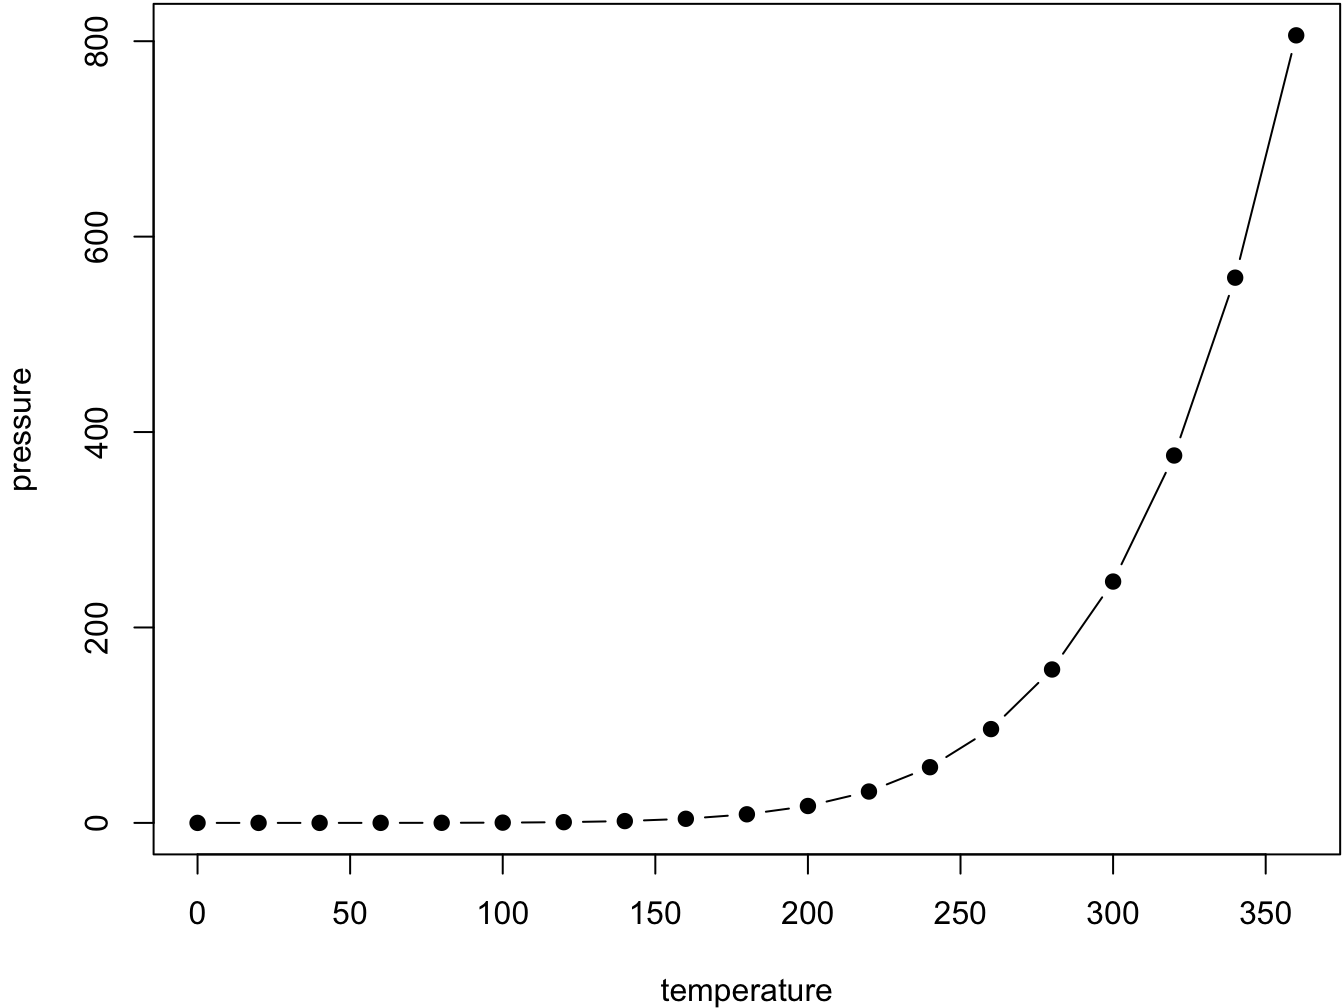
\includegraphics[width=0.8\linewidth]{_main_files/figure-latex/nice-fig-1} 

}

\caption{Here is a nice figure!}\label{fig:nice-fig}
\end{figure}

Don't miss Table \ref{tab:nice-tab}.

\begin{Shaded}
\begin{Highlighting}[]
\NormalTok{knitr}\SpecialCharTok{::}\FunctionTok{kable}\NormalTok{(}
  \FunctionTok{head}\NormalTok{(pressure, }\DecValTok{10}\NormalTok{), }\AttributeTok{caption =} \StringTok{\textquotesingle{}Here is a nice table!\textquotesingle{}}\NormalTok{,}
  \AttributeTok{booktabs =} \ConstantTok{TRUE}
\NormalTok{)}
\end{Highlighting}
\end{Shaded}

\begin{table}

\caption{\label{tab:nice-tab}Here is a nice table!}
\centering
\begin{tabular}[t]{rr}
\toprule
temperature & pressure\\
\midrule
0 & 0.0002\\
20 & 0.0012\\
40 & 0.0060\\
60 & 0.0300\\
80 & 0.0900\\
\addlinespace
100 & 0.2700\\
120 & 0.7500\\
140 & 1.8500\\
160 & 4.2000\\
180 & 8.8000\\
\bottomrule
\end{tabular}
\end{table}

\hypertarget{parts}{%
\chapter{Parts}\label{parts}}

You can add parts to organize one or more book chapters together. Parts can be inserted at the top of an .Rmd file, before the first-level chapter heading in that same file.

Add a numbered part: \texttt{\#\ (PART)\ Act\ one\ \{-\}} (followed by \texttt{\#\ A\ chapter})

Add an unnumbered part: \texttt{\#\ (PART\textbackslash{}*)\ Act\ one\ \{-\}} (followed by \texttt{\#\ A\ chapter})

Add an appendix as a special kind of un-numbered part: \texttt{\#\ (APPENDIX)\ Other\ stuff\ \{-\}} (followed by \texttt{\#\ A\ chapter}). Chapters in an appendix are prepended with letters instead of numbers.

\hypertarget{footnotes-and-citations}{%
\chapter{Footnotes and citations}\label{footnotes-and-citations}}

\hypertarget{footnotes}{%
\section{Footnotes}\label{footnotes}}

Footnotes are put inside the square brackets after a caret \texttt{\^{}{[}{]}}. Like this one \footnote{This is a footnote.}.

\hypertarget{citations}{%
\section{Citations}\label{citations}}

Reference items in your bibliography file(s) using \texttt{@key}.

For example, we are using the \textbf{bookdown} package \citep{R-bookdown} (check out the last code chunk in index.Rmd to see how this citation key was added) in this sample book, which was built on top of R Markdown and \textbf{knitr} \citep{xie2015} (this citation was added manually in an external file book.bib).
Note that the \texttt{.bib} files need to be listed in the index.Rmd with the YAML \texttt{bibliography} key.

The RStudio Visual Markdown Editor can also make it easier to insert citations: \url{https://rstudio.github.io/visual-markdown-editing/\#/citations}

\hypertarget{blocks}{%
\chapter{Blocks}\label{blocks}}

\hypertarget{equations}{%
\section{Equations}\label{equations}}

Here is an equation.

\begin{equation} 
  f\left(k\right) = \binom{n}{k} p^k\left(1-p\right)^{n-k}
  \label{eq:binom}
\end{equation}

You may refer to using \texttt{\textbackslash{}@ref(eq:binom)}, like see Equation \eqref{eq:binom}.

\hypertarget{theorems-and-proofs}{%
\section{Theorems and proofs}\label{theorems-and-proofs}}

Labeled theorems can be referenced in text using \texttt{\textbackslash{}@ref(thm:tri)}, for example, check out this smart theorem \ref{thm:tri}.

\begin{theorem}
\protect\hypertarget{thm:tri}{}\label{thm:tri}For a right triangle, if \(c\) denotes the \emph{length} of the hypotenuse
and \(a\) and \(b\) denote the lengths of the \textbf{other} two sides, we have
\[a^2 + b^2 = c^2\]
\end{theorem}

Read more here \url{https://bookdown.org/yihui/bookdown/markdown-extensions-by-bookdown.html}.

\hypertarget{callout-blocks}{%
\section{Callout blocks}\label{callout-blocks}}

The R Markdown Cookbook provides more help on how to use custom blocks to design your own callouts: \url{https://bookdown.org/yihui/rmarkdown-cookbook/custom-blocks.html}

\hypertarget{sharing-your-book}{%
\chapter{Sharing your book}\label{sharing-your-book}}

\hypertarget{publishing}{%
\section{Publishing}\label{publishing}}

HTML books can be published online, see: \url{https://bookdown.org/yihui/bookdown/publishing.html}

\hypertarget{pages}{%
\section{404 pages}\label{pages}}

By default, users will be directed to a 404 page if they try to access a webpage that cannot be found. If you'd like to customize your 404 page instead of using the default, you may add either a \texttt{\_404.Rmd} or \texttt{\_404.md} file to your project root and use code and/or Markdown syntax.

\hypertarget{metadata-for-sharing}{%
\section{Metadata for sharing}\label{metadata-for-sharing}}

Bookdown HTML books will provide HTML metadata for social sharing on platforms like Twitter, Facebook, and LinkedIn, using information you provide in the \texttt{index.Rmd} YAML. To setup, set the \texttt{url} for your book and the path to your \texttt{cover-image} file. Your book's \texttt{title} and \texttt{description} are also used.

This \texttt{gitbook} uses the same social sharing data across all chapters in your book- all links shared will look the same.

Specify your book's source repository on GitHub using the \texttt{edit} key under the configuration options in the \texttt{\_output.yml} file, which allows users to suggest an edit by linking to a chapter's source file.

Read more about the features of this output format here:

\url{https://pkgs.rstudio.com/bookdown/reference/gitbook.html}

Or use:

\begin{Shaded}
\begin{Highlighting}[]
\NormalTok{?bookdown}\SpecialCharTok{::}\NormalTok{gitbook}
\end{Highlighting}
\end{Shaded}


  \bibliography{book.bib,packages.bib}

\end{document}
